\documentclass{ucbthesis}
\usepackage{biblatex}
\usepackage{amsmath}
\usepackage[pdftex,bookmarks=true]{hyperref}
\usepackage{graphicx}
\usepackage{wrapfig}
\usepackage{listings}
\usepackage{rotating}
\usepackage{makecell}
\usepackage[table]{xcolor}

%\usepackage{wrapfig}
%\renewcommand{\baselinestretch}{2}

% Double spacing, if you want it.
% \def\dsp{\def\baselinestretch{2.0}\large\normalsize}
% \dsp

% If the Grad. Division insists that the first paragraph of a section
% be indented (like the others), then include this line:
% \usepackage{indentfirst}

\newtheorem{theorem}{Jibberish}

\bibliography{references}

\hyphenation{mar-gin-al-ia}

\begin{document}

% Declarations for Front Matter

\title{Automatic Mapping of Real Time Radio Astronomy Signal Processing Pipelines onto Heterogeneous Clusters}
\author{Terry Esther Filiba}
\degreesemester{Fall}
\degreeyear{2013}
\degree{Doctor of Philosophy}
\cochairs{Professor John Wawrzynek}{Daniel Werthimer}
\othermembers{Professor Jan Rabaey \\
  Assistant Professor Aaron Parsons}
\numberofmembers{4}
\prevdegrees{B.S. (University of California, San Diego) 2006}
\field{Engineering -- Electrical Engineering and Computer Sciences}
\campus{Berkeley}

% For a masters thesis, uncomment (remove the % at the beginning of)
% the following line.  This affects the title and approval pages,
% which by default calls this a "dissertation", not a "thesis".

%\itsamasters

% The title page generated by LaTeX is now acceptable for handing in.
% (This was not always the case).

\maketitle
%\approvalpage
\copyrightpage

% (This is included by thesis.tex; you do not latex it by itself.)

\begin{abstract}

% The text of the abstract goes here.  If you need to use a \section
% command you will need to use \section*, \subsection*, etc. so that
% you don't get any numbering.  You probably won't be using any of
% these commands in the abstract anyway.

%CASPER Workshop Abstract


%TODO: This is a copy of the qual abstract, needs to include results, be rewritten

Traditional radio astronomy instrumentation relies on custom built designs, specialized for each science application. 
Traditional high performance computing (HPC) uses general purpose clusters and tools to parallelize the each algorithm across a cluster. 
In real time radio astronomy processing, a simple CPU/GPU cluster alone is insufficient to process the data. 
Instead, digitizing and initial processing of high bandwidth data received from a single antenna is often done in FPGA as it is infeasible to get the data into a single server. 

%In this case, the instrument hardware is not used as general purpose, despite the fact that the FPGAs are reprogrammable.
%Post-processing can easily be done in a CPU or GPU once the FPGA has split up the data into smaller bandwidths or reduced the data. 

%I propose to develop a universal architecture where each problem is partitioned across a heterogeneous cluster, taking advantage of the strengths different technologies have to offer.
%I propose we take an HPC approach to instrument development with a heterogeneous cluster that has both FPGAs and traditional servers.
%This cluster can be reprogrammed as necessary in the same way an HPC cluster is used to run many different applications on the same hardware.

Choosing which platform to use for different parts of an instrument is a growing challenge.
With instrument specifications and platforms constantly changing as technology progresses, the design space for these instruments is unstable and often unpredictable.
Furthermore, the astronomers designing these instruments may not be technology experts, and assessing tradeoffs between different computing architectures, such as FPGAs, GPUs, and ASICs and determining how to partition an instrument  can prove difficult.
In this work, I present a tool called Optimal Rearrangement of Cluster-based Astronomy Signal Processing, or ORCAS, that automatically determines how to optimally partition an instrument across different types of hardware for radio astronomy based on a high level description of the instrument and a set of benchmarks.

In ORCAS, each function in a high level instrument gets profiled on different architectures. 
The architectural mapping is then done by an optimization technique called integer linear programming (ILP). 
The ILP takes the function models as well as the cost model as input and uses them to determine what architecture is best for every function in the instrument.  
ORCAS judges optimality based on a cost function and generates an instrument design that minimizes the total monetary cost, power utilization, or another user-defined cost.

%In order to do this work, I will need to model the platforms and based on a description of the final instrument, generate a processing pipeline.
%The partitioning needs to be done using a variety of techniques to assess the hardware.
%A static model of the hardware is useful to determine the amount of processing available in different types of hardware.
%Dynamic benchmarking would also be needed to deal with varying server architectures and determine how much processing and bandwidth the cpu/gpu servers can handle.
%Finally, to capture any overlooked subtleties or deal with things the tools cannot handle, the user will be able to input hints as to how the instrument should be generated.

%Discussion of actual instruments to develop
% Expand GBT and LEDA, discuss VEGAS
%The development of this tool will be driven by 2 instruments. First, the design of the GBT spectrometer, a spectrometer designed to support many different modes using the same cluster. 
%By using the tool to design this spectrometer, additional modes can be easily added and if the cluster is expanded the each mode can be redesigned to do additional processing that takes advantage of the extra hardware.
%I will also be working on the LEDA correlator. This is a low bandwidth, large N correlator, which is an ideal application for heterogeneous clusters. 

%Discussion of benchmarks
%We can assess the performance of this automatic partitioning tool in a number of ways. 
%First, this tool should significantly reduce NRE and time to science.
%By automatically generating the instrument the need for engineers who understand both science goals and programming is removed. 
%However, this benefit should not come with a large increase in cost.
%The instruments produced by this tool will be compared to optimized implementations with the same parameters on the basis of hardware utilization and power consumption.



%In my thesis, I will look at spectrometers, correlators, and pulsar processors and determine how they could be partitioned across this cluster and benchmark the results. 



%How do we build a radio astronomy instrument compiler. Need to answer 2 questions.

%What does the general purpose architecture look like?
%Traditional radio astronomy designs the complete instrument. Hardware generally not used as general purpose (ie we are using fpgas but rarely reprogram with a new design, just using them so we can share libraries/infrastructure). Need different kinds of architecture to solve most problems (FGPAs, CPUs, GPUs, ASIC)
%Traditional HPC builds a cluster (CPUs and GPUs) and uses tools to run many different algorithms on the same hardware (ie openmp). 
%How do we take the HPC approach for real time radio astronomy processing? Need to design a heterogeneous cluster.

%How do we(the compiler) partition the problem?
%Normal HPC uses homogeneous clusters. How do we deal with an architecture when the nodes are different?
%How do we partition our problem across this heterogeneous cluster?
%What parameters do we need to worry about when compiling for the cluster? Space (keep designs as small as possible freeing hw to run other experiments)? Resolution (maximize the amount of information we get from the data)? Bandwidth (process as much as possible)?

\end{abstract}


\begin{frontmatter}

\begin{dedication}
\null\vfil
\begin{center}
For my parents\\\vspace{12pt}
%TODO
\end{center}
\vfil\null
\end{dedication}

\tableofcontents
\clearpage
\listoffigures
\clearpage
\listoftables

%TODO: Acknowledgements
\begin{acknowledgements}
This work would not have been possible without the help of the people around me.
I am very grateful to my co-advisor Dan Werthimer for his encouragement and mentorship throughout this process.
I appreciate all the time and patience he put in to help me get to this point.
I am also grateful to my co-advisor Professor John Wawrzynek for his guidance which helped motivate me and helped me develop my own research ideas. 
I would like to thank the members of my qual and dissertation committees, Professor Aaron Parsons, Professor Jan Rabaey, and Professor Geoff Bower for their time and help shaping this work.
I also would like to thank Professor Don Backer for his wisdom and support.
Although he is no longer with us, he made a lasting impact on my research and I am very grateful for that.

I also need to thank the members of my research group and my lab.
Thanks to the members of CASPER and the BWRC, especially Mark Wagner, Jonathon Kocz, Peter McMahon, Henry Chen, Matt Dexter, Dave MacMahon, and Andrew Siemion.
I appreciate the time everyone took teaching me, helping me debug things, and discussing my research. 

Finally, I would like to thank the people who looked after me and brightened my time at UC Berkeley.
Thanks to my parents and my sister Michelle for always being around whenever I needed them.
I thank my boyfriend Ben Schrager and his family who welcomed me into their home and treated me like family.
Thanks to my friends Sam Ezell, Rhonda Adato, Leslie Nishiyama, Olivia Nolan, Nat Wharton, Orly Perlstein and Ari Rabkin who kept reminding me that I would eventually finish.
And, I am very grateful for the care I received from my allergist, Dr. James Kong, which made it possible for me to complete this work.

\end{acknowledgements}

\end{frontmatter}

\pagestyle{headings}

% (Optional) \part{First Part}

\chapter{Introduction}



\section{Motivation}

%TODO: Make this prettier
\begin{figure}[ht!]
  \centering
    \includegraphics[width=0.49\textwidth]{Images/C1/vla.png}
    \includegraphics[width=0.49\textwidth]{Images/C1/arecibo.png}
    \includegraphics[width=0.49\textwidth]{Images/C1/paper.png}
  \caption{TODO Telescopes}
  \label{fig: C1/telescopes}
\end{figure}


%TODO: Make this prettier, maybe add a graphic
\begin{figure}[ht!]
  \centering
    \includegraphics[width=0.49\textwidth]{Images/C1/alma_correlator.png}
    \includegraphics[width=0.49\textwidth]{Images/C1/blue_gene.png}
    \includegraphics[width=0.49\textwidth]{Images/C1/vla_correlator.png}
  \caption{TODO Building large systems}
  \label{fig: C1/largesystems}
\end{figure}

%TODO: add some references

\begin{figure}[ht!]
  \centering
    \includegraphics[width=0.49\textwidth]{Images/C1/custom_asic.png}
    \includegraphics[width=0.49\textwidth]{Images/C1/custom_interconnect.png}
  \caption{TODO Building large systems}
  \label{fig: C1/largesystems}
\end{figure}

Traditionally, observatories designed custom instruments that would run on one telescope and solve one problem.
This custom approach was the only way to get the requisite processing power to analyze the radio signals.
This resulted in costly designs, because the boards, backplanes, chips, protocols, and software all needed to be designed from scratch.
To make matters worse, this approach resulted in a very long design cycle,  requiring 5-10 years of development before an instrument could be deployed at a telescope and the time the instrument was released, the hardware would be out of date.

Due to their custom implementations, these instruments also lacked flexibility. 
Each instrument was designed specifically for a single purpose.
This meant upgrading the hardware or modifying the algorithm would require a complete redesign of the instrument, and another long design cycle.


While these older designs needed to trade off flexibility for performance, newer technology can offer both performance and flexibility.
Programmable devices such as FPGAs, GPUs and even CPUs can provide enough processing power to keep up with the data from many new telescopes.
These devices make it easy to reprogram existing hardware to support newer algorithms, and, since they are programmed using portable languages, provide a quick path to upgrade hardware without redesigning the entire instrument.



\section{Challenges}

\subsection{Scientific Challenges}
Radio astronomers are trying to answer a very diverse set of questions. 
%Let�s think about what we�re actually trying to do
%Deal with a diverse set of questions
%Are we alone?
%When were the first stars and galaxies formed?
%Galactic structure and formation (mapping the galaxy)
%Nature of gravitational wave background (pulsar timing)
%Transient universe
%Black hole imaging
%Searching for extrasolar planets

%Number of antennas
%Bandwidth
%Number of channels
%Filter shapes
%Integration time
%Algorithms
%Etc�

%Spectrometer
%Beamformer
%Add signals from multiple antennas together to improve SNR
%Pulsar processor
%Detect dispersed pulse
%Interferometer/correlator
%Cross-correlate signals from many antennas to combine into a spectral image
%Increase angular resolution

%Spectrometer
%Filter bank/FFT
%Accumulation
%Beamformer
%FFT
%Phase shift
%Adders
%Pulsar processor
%FFT
%Deconvolution
%Interferometer/correlator
%FFT
%Cross correlation (multipliers)
%Accumulation

\subsection{Technological Challenges}

%Large number of small antennas to improve sensitivity and resolution
%Small antennas are very low cost
%Creates very high performance signal processing requirements
%Need to combine the antennas together to form a single image or beam
%Interferometry computation requirements scale as N2 (N = number of antennas) ~100Tops

\begin{figure}[ht!]
  \centering
    \includegraphics[width=\textwidth]{Images/C1/design_space.pdf}
  \caption{TODO}
  \label{fig: C1/design_space.pdf}
\end{figure}

%Increasing
%
%Design time
%
%Design complexity
%
%Performance
%
%Cost (in low volume)
%
%Decreasing
%
%Power (watts)
%
%Flexibility




%Assessing tradeoffs
%3 GHz bandwidth
%100-200 MHz bandwidth
%Fixed point
%Floating point
%Streaming designs
%Conditional/Iterative programming
%Difficult to program (HDL)
%Easy to program (CUDA)
%Difficult to achieve peak performance
%Difficult to achieve peak performance
%$$
%$
%Lots of available IO
%Limited IO

%Zooming in on the middle of the spectrum, a lot of other things to consider
%Options for reprogrammable architecture
%Floating point can be good or bad depending on the application, some can get away with very small bit widths

%Traditional instrument design
%Traditionally observatories build custom instruments
%High cost due to custom designed 
%boards
%backplanes
%chips 
%protocols
%software
%Development takes 5 to 10 years
%Hardware is out of date by the time it�s released
%Difficult to upgrade/modify without a redesign

%A number of options are available but which is best?
%Need to understand how to choose the right platform(s) for each implementation
%With constant changes in technology and algorithm implementations an automatic approach is required

\section{ORCAS}



 
\chapter{Radio Astronomy Instrumentation}
%Summary: Give an description of radio astronomy instrumentation \\
%Describe science goals and mathematical function \\
%Goal: Give background for the application. Show that most instruments use a small number of high level functions\\
%State: Can be written now \\
%Use info from casper papers and radio 101 \\
%References already compiled \\

\section{Science Goals}
\section{Algorithms}
\subsection{Spectroscopy}
\subsection{Pulsar processing}
Detect dispersed pulses
\subsection{Beamforming}
Add together multiple (delayed) signals to improve SNR
\subsection{Interferometry}
Form an image
 
\chapter{Related Work} \label{Related Work:Radio Astronomy}
%Summary: 2 major sections, 1 about past radio instrumentation, 1 about automatic mapping\\
%Goal: Explain why we can mesh them together successfully in this case\\
%State: Can be written now \\
%List of references already compiled into Papers archive \\

%TODO: Intro
\section{Radio Astronomy} \label{Related Work:Radio Astronomy}
%\subsection{Digital Signal Processing for Radio Astronomy}
The need for high bandwidth processing manifests in many different radio astronomy applications.
Keeping up with increasing computation demands has often resulted in the specialized design of spectrometers.

%TODO: Intro
\subsection{Distributed FX Correlator (DiFX)}

\begin{figure}[ht!]
  \centering
    \includegraphics[width=\textwidth]{Images/C3/vlba.pdf}
  \caption{Telescope Locations in the Very Long Baseline Array}
  \label{fig: C3/vlba.pdf}
\end{figure}

The Very Long Baseline Interferometery or VLBI technique uses an array of antennas that are extremely far apart to achieve very high angular resolution. 



\begin{figure}[ht!]
  \centering
    \includegraphics[width=\textwidth]{Images/C3/difx_architecture.pdf}
  \caption[DiFX Correlator Architecture]{DiFX Correlator Architecture (reprinted from \citeauthor{Deller:2007wy} \cite{Deller:2007wy})}
  \label{fig: C3/difx_architecture.pdf}
\end{figure}

%DiFX (Distributed FX Correlator) is a scalable software implementation
The DiFX Correlator is a scalable software implementation of an FX Correlator  \cite{Deller:2007wy}.
DiFX was designed as a software correlator that targets CPUs in order to maintain flexibility in the design, but that flexibility comes at a high hardware cost. 
%Requires a large cluster to do a lot of computation
%64 MHz, 10 antennas required ~100 nodes in 2007
Nearly 100 nodes are required to cross correlate 64 MHz of bandwidth from 10 antennas. 
%TODO: define expensive
%TODO: define the nodes more precisely

%TODO: If you have a cluster available�
%Why do cpu-only?
%It�s easy
%Compared to 27 antenna 2GHz EVLA in New Mexico

The correlator was originally developed to do VLBI (Very Long Baseline interfereometery). 

%TODO: expand on VLBI
%TODO: doesn't need to be real time (using recorded data)

%Designed for VLBI (Very Long Baseline Interferometry)

\subsection{LOFAR}
\begin{figure}[ht!]
  \centering
    \includegraphics[width=\textwidth]{Images/C3/lofar_performance.pdf}
  \caption[LOFAR Correlator Performance]{LOFAR Correlator Performance (reprinted from \citeauthor{vanNieuwpoort:2009p1253} \cite{vanNieuwpoort:2009p1253})}
  \label{fig: C3/lofar_performance.pdf}
\end{figure}
%On a blue gene, real time but still costly power hungry solution 64 stations
%TODO: read this paper
Like DiFX, the correlator for Low-Frequency Array for Radio Astronomy (or LOFAR) was also built using CPUs \cite{vanNieuwpoort:2009p1253}.
This project used a Blue Gene BG/P %TODO: check this
to implement a 64 station correlator.
The implementation got very high performance out of the cluster, 96\% of the peak, but required an entire cluster and required finely tuned code to achieve that performance. 


\subsection{xGPU}
xGPU is a CUDA package that implements the cross-correlation
%TODO: add another graph from paper
\begin{figure}[ht!]
  \centering
    \includegraphics[width=\textwidth]{Images/C3/gpuxperformance.pdf}
  \caption[xGPU Performance]{xGPU Performance (reprinted from \citeauthor{Clark:2011wi} \cite{Clark:2011wi})}
  \label{fig: C3/gpuxperformance.pdf}
\end{figure}

\cite{Clark:2011wi}

\cite{2009PASP..121..857W}


\subsection{CASPER}

At the Collaboration for Astronomy Signal Processing and Electronics Research (CASPER), we are developing  common libraries and hardware that can be used by radio astronomers developing instrumentation. The mission statement, available on the website, concisely summarizes the goals of the group:

\begin{quotation}
The primary goal of CASPER is to streamline and simplify the design flow of radio astronomy instrumentation by promoting design reuse through the development of platform-independent, open-source hardware and software.
Our aim is to couple the real-time streaming performance of application-specific hardware with the design simplicity of general-purpose software. By providing parameterized, platform-independent "gateware" libraries that run on reconfigurable, modular hardware building blocks, we abstract away low-level implementation details and allow astronomers to rapidly design and deploy new instruments.
\end{quotation}

The collaboration, started at UC Berkeley by Dan Werthimer, Don Backer, and Mel Wright, has spread to include astronomers all over the world, as shown in Figure \ref{fig: C3/casper_collaborators.png}. 
The group collaborates with many large digital engineering groups including groups from the Jet Propulsion Laboratory (JPL), the National Radio Astronomy Observatory (NRAO), the Arecibo Observatory, SKA South Africa, and the Giant Metrewave Radio Telescope (GMRT) in India. 
The diversity and far reach in this collaboration ensures that the tools continue to be general purpose and widely accessible. 


\begin{figure}[h!]
  \centering
    \includegraphics[width=\textwidth]{Images/C3/casper_collaborators.png}
  \caption{Map of CASPER Collaborators}
  \label{fig: C3/casper_collaborators.png}
\end{figure}

The CASPER FPGA libraries were developed to mitigate the need to redevelop common signal processing blocks for every new instrument \cite{Parsons:2006cu}. 
The library provides parameterized blocks such as FFTs, digital down-converters, and FIR filters that are the necessary building blocks for a wide range of instruments. 
Coupled with open source FPGA boards, such as the ROACH (Reconfigurable Open Architecture Computing Hardware), the CASPER libraries provide a useful toolbox for radio astronomy instrumentation development.
The follow sections describe each of these and how they have been used to create a number of different instruments.



\subsubsection{CASPER Hardware}

The CASPER group provides set of modular FPGA boards and ADCs that are designed specifically to deal with the high bandwidth requirements of real time radio astronomy signal processing. 
Since each FPGA boards meets the needs of the radio astronomy community as a whole rather than a single application, the group releases a small number of boards and typically only releases a new board to take advantage of improving technology. 
The CASPER library and software, discussed below, also make it easy to upgrade the hardware since a CASPER design easily be recompiled to work with a different board and the software interface and the signal processing model are standardized.
And, since the boards communicate over a common set of industry standard protocols, they can be upgraded one by one, or all at once. 

Each FPGA board implements a number of high speed interfaces to send and receive data.
The Z-DOK+ connectors are primarily used to interface the boards to high speed ADCs and DACs.
This common Z-DOK+ interconnect implemented on nearly all CASPER ADC boards allows the astronomer to choose an ADC to match their scientific goals. 
The diversity of available boards is shown in Table \ref{tab: C3/adcs}.

\begin{table}
\centering
\begin{tabular}{| l | l | l | l |}
\hline  
\textbf{ADC Name} & Max sample rate & Streams & Bitwidth \\
\hline  
64ADCx64-12 & 50 Msps & 64 & 12 bits\\
ADC4x250-8 or QuadADC & 250 Msps & 4 & 8 bits\\
KatADC & 1.5 Gsps & 1 & 8 bits  \\
ADC1X2200-10 & 2.2 Gsps & 1 & 10 bits \\
ADC1x10000-4 & 10 Gsps & 1 & 4 bits \\
\hline  
\end{tabular}
\caption{CASPER ADC Comparison}
\label{tab: C3/adcs}
\end{table} 



%TODO: Provides tested hardware for new instruments

Each board can also send or receive data using ethernet. 
The boards are designed to communicate using common protocols, like 10GbE, so a board can be upgraded without modifying how it communicates with the rest of the cluster. 
The use of an industry standard protocol also makes communication to non-CASPER boards simple, allowing an FPGA to create UDP packets that eventually get received by a CPU or GPU-based server, making the CASPER boards an ideal component in a heterogeneous cluster. 
This makes it simple to design a cluster, and allows continuous upgrades as technology improves, as the signal processing model and communication model do not change between boards.


%All boards can talk to each other
%Can�t clock FPGA at 3GHz but use parallel FFT 8-16 samples at a time
%BEE2 lib w/Bob Broderson

%TODO: add roach 2, bee2, ibob
\begin{figure}[ht!]
  \centering
    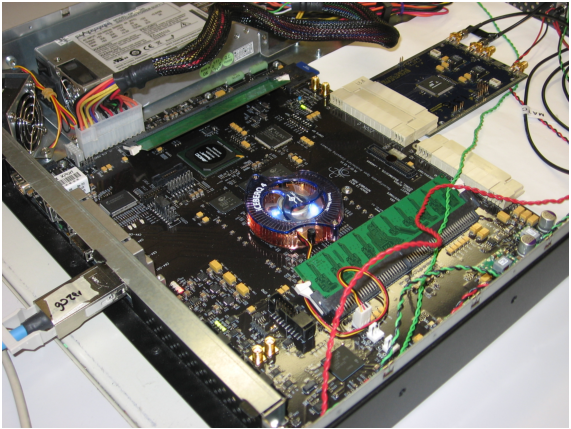
\includegraphics[width=\textwidth]{Images/C3/roach.pdf}
  \caption{ROACH Board}
  \label{fig: C3/roach.pdf}
\end{figure}

The ROACH board, shown in Figure \ref{fig: C3/roach.pdf}, with an iADC board connected via Z-DOK+ and an ethernet cable to get data off the board. 
%TODO: expand



\subsubsection{CASPER Library}

%TODO: edit this
CASPER develops a DSP library that can be compiled into an FPGA bitstream.
The library is implemented in Simulink, which allows for both simulation and, using Xilinx System Generator, compilation to FPGA code.
The Simulink designs can be retargeted to different boards without changed the original implementation.
%TODO: discuss simulink, visual programming, etc

%  Platform independent DSP library
%  Blocks can be used on any CASPER board (BEE2 or iBOB,
%ROACH coming soon...)
%  Currently restricted to Xilinx chips but can be ported to other platforms
%  Large set of parameterizable DSP building blocks
%  FFTs (tunable bandwidth, number of channels, real or complex) ?  PFBs
%  Accumulators
%  All library blocks are built from Xilinx primitive blocks
%  Matlab scripts (�mask scripts�) are used to configure parameterized blocks

%CASPER = Collaboration for Astronomy Signal Processing and Electronics Research
%Identifies commonly used DSP blocks for radio astronomy
%FFTs (tunable bandwidth, number of channels, real or complex)
%Polyphase filter banks
%Accumulators
%Digital downconverters/mixers
%Scripts are used to configure parameterized blocks

\begin{figure}
  \centering
     \includegraphics[width=\textwidth]{Images/C3/casper_fft_lib.pdf}
  \caption{CASPER FFT Library}
  \label{fig:casper_fft_lib.pdf}
\end{figure}

%TODO: remove this is achieved by
The CASPER library includes commonly used DSP blocks in radio astronomy instruments.
For example, the CASPER library provides FFTs, FIR filters, accumulators, digital downconverters, digital mixers which can be linked together to make an instrument. 
Each block is parameterized, making them useful for a variety of instruments. 
Figure \ref{fig:casper_fft_lib.pdf} shows the FFT library, which contains different types of FFTs, including blocks that can process multiple samples in parallel and blocks that are optimized to compute the FFT of a real signal. 


\begin{figure}
  \centering
     \includegraphics[width=0.45\textwidth]{Images/C3/casper_fft_lib_options.pdf}
  \caption{CASPER FFT Options Menu}
  \label{fig:casper_fft_lib_options.pdf}
\end{figure}


Figure \ref{fig:casper_fft_lib_options.pdf} shows the options menu for one of the FFT blocks. 
In order to support a variety of instruments, this block can be reconfigured to support different FFT lengths.
There are a number of other parameters provided like input bit width, which helps support a number of different ADCs or preprocessing algorithms, and FPGA-specific parameters like add latency, and multiply latency which have no effect on the result of the computation but change how the FFT gets mapped into hardware. 

\begin{figure}[ht!]
  \centering
    \includegraphics[width=0.48\textwidth]{Images/C4/fft_response.png}
    \includegraphics[width=0.48\textwidth]{Images/C4/pfb_response.png}
  \caption{A comparison of FFT and PFB response}
  \label{fig: fft_vs_pfb_response}
\end{figure}

PASP uses a PFB to split up the subbands. Figure \ref{fig: fft_vs_pfb_response} shows a comparison between the FFT and PFB response. 
The FFT response (on the left) has a lot of spectral leakage while the PFB (on the right) has a much sharper filter shape and a better frequency response. 
The superior frequency response led us to use a PFB rather than an FFT to extract subbands, despite the additional FPGA resources required by the FIR filter before the FFT.

\begin{figure}[ht!]
  \centering
    \includegraphics[width=0.49\textwidth]{Images/C3/adder_tree_diagram.pdf}
    \includegraphics[width=0.49\textwidth]{Images/C3/adder_tree_code.pdf}
  \caption{Adder Tree Simulink Diagram and Code}
  \label{fig: C3/adder_tree}
\end{figure}


These parameters in the options menu are implemented using a number of matlab scripts to automatically design the block. 
%TODO: expand on this


%TODO: maybe break this down into separate blocks
\begin{figure}
  \centering
     \includegraphics[width=0.75\textwidth]{Images/C3/yellow_blocks.pdf}
  \caption{TODO}
  \label{fig:C3/yellow_blocks.pdf}
\end{figure}

The CASPER library also provides a set of blocks to abstract away the implementation of I/O interfaces, which are called yellow blocks. 
Figure \ref{fig:C3/yellow_blocks.pdf} provides some examples of what those library blocks look like. 
Each block provides input and output ports that correspond to the data it can send or receive. 
For example, the adc block has an output ports labeled \emph{o0,o1,\ldots,o7} that represent the data the FPGA receives from the iADC board.
In addition to this, simulation ports are provided to allow the user to proved test signals mimicking the outside world.
In the case of the adc, the user could provide a sine wave into the \emph{sim\_in} port to observe how a sine wave would be processed by the system.
During compilation, the CASPER XPS toolflow automatically processes the blocks and ensures the wires are connected to the correct pins.

%TODO: discuss debugging with yellow blocks


\subsubsection{CASPER Software}

%Toolflow for compilation, ref BEE2 compile path, borph, etc
To simplify the use of the FPGA further, the CASPER boards run a modified version of Linux directly on the board. 
Using this Linux environment, called the Berkeley Os for ReProgrammable Hardware or BORPH, programming the FPGA is as simple as running an executable on the command line \cite{So:2007ve}.
Then, once the board has been programmed, BORPH can communicate with the chip using an interface where components on the FPGA like registers or memory appear as a file system in the operating system. 
These files can be accessed using normal file I/O, making it simple to send control signals or monitor the status of the chip.

\cite{Cross:2009ta}

\subsubsection{SERENDIP V.v}

\begin{figure}[ht!]
  \centering
    \includegraphics[width=\textwidth]{Images/C3/setispectrometerv55.pdf}
  \caption{SERENDIP V.v Block Diagram}
  \label{fig: C3/setispectrometerv55.pdf}
\end{figure}

%Used for the SETI ALFA Survey, JPL Sky Survey, and Argentina SETI
%  200 MHz Bandwidth currently, future plans to upgrade to 300MHz
%  128 Million frequency channels
%  Build using an iADC, iBOB and BEE2
%  Can process one polarization from a single beam

\begin{figure}[ht!]
  \centering
    \includegraphics[width=\textwidth]{Images/C3/alfa_feed.png}
  \caption{Arecibo ALFA Feed}
  \label{fig: C3/alfa_feed.png}
\end{figure}

\begin{figure}[ht!]
  \centering
    \includegraphics[width=0.48\textwidth]{Images/C3/serendip_vv_top.png}
    \includegraphics[width=0.48\textwidth]{Images/C3/serendip_vv_bottom.png}
  \caption{SERENDIP V.v Hardware installed at Arecibo Observatory}
  \label{fig: C3/serendipvv}
\end{figure}

%4k point PFB
%  32k by 4k corner turn
%  32k point FFT
%  Each element (PFB, corner turn, FFT, and thresholder) is on a separate BEE2 chip
%  Output to PC is low bandwidth due to thresholding
%  Upcoming ROACH architecture will support 2 polarizations, 400 MHz

%SuccessfullydeployedatAreciboObservatoryinJune2009
%  ImplementedonanIBOBandBEE2board
%  200MHzbandwidth
%  28million(227)channels(4kcoarsechannels*32kfinechannels)
%  1. 5 Hz/channel
%  0. 67 sec integration time
%  ObservescommensallywithallALFAobservations
%  Observesonlyonebeamatatime

%Arecibo L-band Feed Array
%?  7 pixel dual polarization ?  ALFA RF 1225-1525 MHz

\cite{2010LPICo1538.5378S}


\subsubsection{CASPER Correlator}
\begin{figure}[ht!]
  \centering
    \includegraphics[width=\textwidth]{Images/C3/casper_correlator.png}
  \caption{CASPER Correlator Block Diagram}
  \label{fig: C3/casper_correlator.png}
\end{figure}

\cite{Parsons:2008dl}

%Used to develop Parsons/Manley correlator
%10GbE switch solves cabling problem
%Still have N^2 X engines

\section{Tuning} \label{Related Work:Tuning}
\subsection{Metropolis}

The Metropolis project focused on mapping algorithms onto embedded systems \cite{Davare:2007ue}. 
The tool provides a framework for an abstract block based description of the algorithm. 
This description makes it easy to stitch algorithms together without specifying the eventual hardware implementation, providing a simple path to simulation and algorithm development that is separate from the implemented design. 
Then, the tool automatically maps the description onto an existing heterogeneous embedded system. 

%TODO: review references
\cite{Balarin:2003kc}
\cite{Densmore:tm}

%Mapping is focused on scheduling onto heterogeneous platforms
%Strong focus on embedded systems

%Some people have thought about how to use technology
%Metropolis works on simulation extensively (supporting 
%Embedded systems � we have 1 cpu and 1 dsp let�s make it go fast
%This doesn�t solve our problem
%Just does scheduling

The mapping generated by the tool is simply a schedule, specifying where and when each part of the computation gets executed. 
The tool seeks to optimize performance of the algorithm, ensuring the generated schedule runs as fast as possible on the hardware provided. 
This technique requires a fixed hardware model and uses the existing hardware to optimize performance. 
While this work is useful when a hardware model exists, it does not provide any flexibility in the hardware model while mapping the algorithm. 
So, when it is necessary to design the hardware to begin with, this does not solve the problem. 

%Doesn�t help design the cluster
%A �heterogeneous node� has a fixed mix of resources
%Can�t reduce costs by throwing away certain types of hardware
%Optimization is based on a fixed architecture and flexible performance
%Doesn�t match our �always running� model
%Performance is �good enough�, not an optimization target

Additionally, this type of solution is ill-suited to mapping the algorithms required to do real-time radio astronomy signal processing. 
This tool assumes it must schedule a discrete task onto a fixed piece of hardware and attempts maximize the performance of the task. 
In the applications described in Chapter \ref{chap:Real Time Radio Astronomy Algorithms}, the computation should always be running and needs to meet some minimum performance target.
Once the performance target is met, it is better to have a tool that will other costs like power or amount of hardware, rather attempting to improve the runtime of the algorithm. 








%Lisa Marie Guerra (?)


\subsection{Scheduling}
An integer linear programming model for mapping applications on hybrid systems

%TODO: sort these out
\cite{Gibeling:2008vg}

\cite{Theodoridis:2009gd}

\cite{Tsoi:2010we}

\cite{Jun:2008vv}

\cite{Rakhshanfar:2011tg} 
\chapter{High Level Toolflow}
%Summary: Introduce idea of end to end toolflow
%Goal: Defend the idea that we can design an instrument using only a simple high level specification
%1
%State: Can be partially written now
%The end description will likely change based on the partitioning results

%Summary: describe CASPER, PASP and reconfigurable heterogeneous setispec Goals:
%describe the existence and continued development of �blocks�
%show the ability to design reconfigurable instruments by adding a layer of abstraction to the CASPER+xgpu work
%State: Can be written now
%Content already exists in the form of talks and a short paper.






%TODO: Place
%Cluster abstraction
%Treat platforms as cluster nodes
%Assume all platforms elements are attached to a switch
%Assume a full crossbar network
%Fully connected network
%Often necessary in radio astronomy
%Try to determine the best mapping based on some cost metric

%A number of options are available but which is best?
%Need to understand how to choose the right platform(s) for each implementation
%With constant changes in technology and algorithm implementations an automatic approach is required




\section{Toolflow Goals} \label{High Level Toolflow:Toolflow Goals}

%Describe what the tool flow should to, for whom, etc

%Ideal instrument design
%Buy technology at the last minute
%Ensure we get the best price for the performance we need
%Choose hardware based on cost ($, watts, rack space)
%Low instrument development time
%Assess impacts of potential optimization without implementing anything
%Quickly assess performance on new or nonexistent technology
%Reduce debugging time on new platforms
%Support whatever hardware is currently most appropriate

%Goals
%Interface
%Accessible to astronomers (domain experts)
Ideally, this tool should be accessible to both computer experts and radio astronomers, or other domain experts.
For a domain expert, the tool should allow someone to define the algorithm they need without worrying how it will ultimately map to hardware.
%Accessible computer experts
%Implementation
%Generate code for an instrument optimally mapped across a heterogeneous cluster
%Retain improvements offered by low-level optimization
The computer expert should be able to define the algorithm, but also needs some means for providing optimization.
For example, if an engineer wrote an optimized FFT algorithm, the tool will be able to incorporate that into the final optimized result.
And in the end, Regardless of who is using this tool, an optimal mapping of the algorithm gets produced. 
Because the needs of these groups are so different, Sections \ref{High Level Toolflow:Instrument Definition} and  \ref{High Level Toolflow:Dataflow Model} will describe how this is addressed at different steps in the tool flow.





\section{Instrument Definition} \label{High Level Toolflow:Instrument Definition}
%Describe instrument using parameters an astronomer can understand
%Small number of predefined instrument types
%Need to input
%Instrument type (predefined patterns)
%Total Bandwidth
%Array size (n)
%Etc
%Generates a dataflow representation
At the first step in the toolflow, the user must describe the instrument using high level parameters. 
These parameters should all 


\section{Dataflow Model} \label{High Level Toolflow:Dataflow Model}

%Dataflow representation of instrument
%Define input/output connections
%Define input/output bandwidth
%Generates a series of blocks configured to talk to each other

\subsection{Computational Blocks}
%Collection of blocks necessary to solve most problems
%Can be parameterized
%Include a method to assess performance on each (supported) platform
%Performance model
%Benchmark
%Unit tests
%Uniform interconnect model
%Optimization: remove interconnect overhead for cores running on the same hardware

%Not certain this belongs here, possibly should go with the models?
%Before mapping, need to determine which blocks can be mapped to which platforms
%Synthesize/compile existing implementations to determine which platforms can support the spec
%Sanity check bandwidth requirements
%Test for acceptable noise tolerance in different implementations
%Known signals
%Test against arbitrary precision (exact) floating point implementation


\subsection{Connection Types}

Suppose we know we have 2 types of blocks: $A$, and $B$. 
Blocks of type $A$ must send their output to blocks of type $B$.
Now, we need to understand how blocks of type $A$ send data to blocks of type $B$.
This could happen in 2 ways, `one-to-one' and `all-to-all'. 

\begin{wrapfigure}[18]{l}{0.37\textwidth}
  \centering
    \includegraphics[width=0.35\textwidth]{Images/C5/one-to-one.pdf}
  \caption{TODO}
  \label{fig:one-to-one.pdf}
\end{wrapfigure}

A `one-to-one' connection is where every block of type $A$ communicates with exactly one block of type $B$, as shown in Figure \ref{fig:one-to-one.pdf}. 
With this type of connection, the number of blocks of type $A$ must be equal to the number of blocks of type $B$.
The F-engines in a FX correlator are a good example of this type of connection. 
The correlator has an F-engine for each antenna, each containing the same blocks linked in the same way. 
Within an F-engine, a PFB\_FIR filter must communicate with a single FFT.
In general, every PFB\_FIR within an F-engine, blocktype `A' must communicate with exactly one FFT, blocktype `B'. 



\begin{wrapfigure}[18]{r}{0.47\textwidth}
  \centering
    \includegraphics[width=0.45\textwidth]{Images/C5/all-to-all.pdf}
  \caption{TODO}
  \label{fig:all-to-all.pdf}
\end{wrapfigure}
      



An `all-to-all' connection occurs when every block of type $A$ must send some data to ever block of type $B$. 
Figure \ref{fig:all-to-all.pdf} shows what an all-to-all connection between 3 blocks of type $A$, and 3 blocks of type $B$ will look like. 
In this case, every block of type $A$ must send some data to every block of type $B$. 
For example, the type of connection between the per-antenna FFTs and the per-channel X-engines in an FX correlator would be `all-to-all'. 
Each X-engine needs a small amount of data from every F-engine to compute the cross-correlations from a single channel. 
In the `all-to-all' case, there is no reason for the number of sending nodes needs to be the same as the number of receiving nodes. 
%The n's do not get introduced until the ILP is defined
%This means that $n_{i,A}$ and $n_{i,B}$ do not have to be equal, and as long as the data can be distributed appropriately, there is no enforced relationship between the two variables. 




%TODO: make this an a,b figure
\begin{wrapfigure}{r}{0.47\textwidth}
  \centering
    \includegraphics[width=0.4\textwidth]{Images/C5/one-to-all.pdf}
    \includegraphics[width=0.4\textwidth]{Images/C5/all-to-one.pdf}
  \caption{TODO}
  \label{fig: one-to-all_vs_all-to-one}
\end{wrapfigure}



It might seem like there are two more possible types of connection, `one-to-all' and `all-to-one' .
A data flow with a `one-to-all' connection, shown in Figure x %TODO: fix reference, image
would have exactly one block of type $A$ that needs to send data to many blocks of type $B$. 
This is exemplified in the dataflow for a high-resolution spectrometer.
The coarse channelization is done in a single FFT block, which then needs to send the data to many other FFTs to do the fine channelization. 
The `all-to-one' connection shown in Figure x %TODO: fix ref
is there reverse of the `one-to-all' case. 
In this type of connection, there are many blocks of type $A$ and they all need to send data to a single instance of a block of type $B$. 
An example of this arises when some processing is done in a distributed manner but the instrument needs to record the final result in a central place. 
The $A$ blocks are responsible for the distributed processing, and then the $B$ block needs to collect the results and combine them.
%TODO: discuss scatter-gather?

It turns out, these are both special instances of the `all-to-all' connection. 
The `one-to-all' connection is simply an `all-to-all' where the number of $A$ blocks is fixed at 1.
Similarly, the `all-to-one' connection is also an `all-to-all' where the number of $B$ blocks is fixed at 1.
Because of this, there is no need to include or support these cases as unique connection types. 


While it may seem like additional link types exist like `all-to-some' or `one-to-some', this turns out to be impossible. 
Either a block of type $A$ cannot send its data to only some blocks of type $B$ because of the way blocktypes are defined.
Any block of the same type should be interchangeable with another block of the same type.
In an `all-to-some' connection, blocks of type $A$ would need to send data to $B_1$ but not send data to $B_2$.
But that connection patterns implies that the blocks $B_1$ and $B_2$ are \emph{not} interchangeable and therefore cannot have the same blocktype.


%TODO: This isn't implemented in the ILP
%TODO: Add correlator beamformer example. 
This does not preclude asymmetrical designs. 
Instead, asymmetry is supported by allowing blocks to define a list of blocktypes they must send data to or receive data from. 
The connection between any two blocktypes still must be described as above.

\subsection{Case Studies}


%TODO: think hard about this, we're not actually going to do this and it's optional
%This could be a good place to describe PASP, this is doable, we've shown it's possible
%Don't actually want to implement the entire thing but show feasibility
\section{Optional: Code Generation}
%Use a mapped dataflow to stitch together blocks
%To generate code the blocks must have an implementation for the target platform (not necessary for mapping)
%Include an automatic test suite for each platform
%Block communication is standardized so they can be connected in arbitrary ways



%TODO: This will likely be moved elsewhere, including it here temporarily
\pagebreak


\section{Instrument Generation}
%From USRI 2011 paper
Automatic Generation of Heterogeneous Spectrometers for Radio Astronomy

We have developed a software package to automatically generate spectrometers with minimal user input.
Spectrometer design is often done by building the instrument from scratch.
We have automated this design, creating a parameterized spectrometer that only requires a recompile to implement a change in specification.
This spectrometer combines FPGAs and GPUs, doing coarse channelization on the FPGA and sending each subband to the GPUs for further processing.
The server software is designed for flexibility, allowing astronomers to easily modify the processing algorithm run on the GPU and customize the instrument to fit their science goals.

\section{Introduction}
The need for high bandwidth spectroscopy manifests in many different radio astronomy applications.
Keeping up with increasing computation demands has often resulted in the specialized design of spectrometers.
At the Collaboration for Astronomy Signal Processing and Electronics Research (CASPER), we have developed a software package to automatically generate spectrometers for a variety of applications.

The CASPER FPGA libraries were developed to mitigate the need to redevelop common signal processing blocks for every new instrument \cite{Parsons:2009vc}. 
Parameterized blocks such as FFTs and digital down-converters can easily be used to design many different instruments. 
Coupled with open source FPGA boards, such as the ROACH (Reconfigurable Open Architecture Computing Hardware), the CASPER libraries provide a useful toolbox for radio astronomy instrumentation development.
This work extends the CASPER philosophy, demonstrating that entire instruments can be generated with minimal user input.
Rather than designing a completely different instrument for every different specification, this software package is parameterized so a change in specification only requires a recompile.

The software package includes an FPGA design and server software to do spectroscopy, as well as server benchmarks used to determine an optimal instrument configuration.
%The benchmarks measure maximum amount of data the servers can process, determining the optimal configuration for the instrument.
Both the FPGA and server software are parameterized, allowing for rapid deployment of a working spectrometer that is configured to take full advantage of available computing resources.
%Our general purpose approach allows for the rapid development of new instruments.
We implement the instrument on a heterogeneous cluster consisting of both FPGAs and GPUs to take advantage of the benefits provided by both platforms.
FPGAs provide high bandwidth processing but can be cumbersome to program.
GPUs can't handle the same bandwidths as FPGAs but they are easier to program. 
The CUDA language, for example, is a C-like language that can be used to develop software for many GPUs.
The high level parameters in this package allow us to use FPGAs while abstracting away implementation details specific to the FPGA.
To give the user control over their data processing algorithm, an application specific GPU program can be written and easily interfaced with the existing receive software in the package.
%Heterogeneous clusters 

\section{Radio Astronomy Applications}
This instrument has a wide variety of potential applications due to the flexibility of the server software. 
In this section, we describe a few specific applications than can make use of this package.

In the search for extraterrestrial intelligence (SETI), the ability to keep up with changes in technology allows searching instrumentation to stay on the leading edge of sensitivity. 
SETI aims to process the maximum bandwidth possible with very high resolution spectroscopy.
This instrument allows SETI projects to easily keep up with improvements on the telescope and increasing computational power.
An increase in detector bandwidth, improving the breadth of the search, can be processed simply recompiling the FPGA design and distributing the extra subbands to new servers. 
As computation improves, the instrument can be reconfigured to send more bandwidth to each computer, reducing the required cluster size, or improve the resolution of the instrument by doing a larger FFT on the server.

This design also has applications in pulsar science. 
The fast channelization on the FPGA with no data reduction makes it an ideal pulsar spectrometer, since no information is lost before sending the data to the servers.
GPUs provide a good platform for pulsar processing algorithms such as coherent dedispersion \cite{Ransom:2009wz}, which can easily be used as the processing function for the server software distributed in our package. 
Similar to SETI instruments, pulsar instruments designed using this package can also keep up with improvements in technology with a simple recompile.


\section{Instrument Architecture}
The instruments generated with this package use a heterogeneous design, allowing us to benefit from the strengths of FPGAs and GPUs. 
The FPGA board is able to sample and process very high bandwidths that a single CPU or GPU would not be able to manage; 
once the FPGA has split up the band the GPU provides a platform that is easier than an FPGA to program but still provides high compute power. 
A design called the Packetized Astronomy Signal Processor, or PASP, is run on the FPGA.
PASP splits up the large band into smaller bands that can be processed using off the shelf servers.
The subbands are put into packets on the FPGA and sent over a 10 gigabit Ethernet switch to a cluster of servers.
The servers receive the data from the switch and process it using spectroscopy software provided in the software package or special purpose application software written by the user and linked into the provided packet processing infrastructure.

Figure \ref{fig:spec_highlevel} shows a high level view of a spectrometer that could be designed with this package. 
In this example, a ROACH board divides the input band into 64 subbands and sends them out to a 16 server cluster.
An ADC is used to digitize data from the telescope and connects to the ROACH board via Z-DOK connectors. 
The digitized data is split into 64 subbands and sent through a 10 gigabit Ethernet switch.
Each server in the cluster receives and processes 4 subbands.

\begin{figure}[ht!]
  \centering
     \includegraphics[width=1\textwidth]{Images/C4/spec_highlevel.png}
  \caption{Example high level instrument architecture}
  \label{fig:spec_highlevel}
\end{figure}


\subsection{FPGA Design}

%TODO : stuff about the pasp design here

Figure \ref{fig: pasp_fpga_arch} gives an overview of the dataflow through the FPGA.
The FPGA interfaces to a single ADC board that simultaneously digitizes 2 signals. 
Each signal can be sampled at a maximum rate of 1Msps.
The samples are sent into a polyphase filter bank (PFB), consisting of an FIR filter and an FFT, which breaks up the entire bandwidth sampled by the ADC into smaller subbands.
After dividing up the subbands, each band is rescaled. 
This step allows us to compensate for the shape of the analog filter feeding data into the ADC. 
After rescaling, the FPGA forms packets where each packet contains data from a single subband. %TODO fix
The packets are sent out over CX4 ports to a 10 gigabit Ethernet switch.

\begin{figure}[ht!]
  \centering
    \includegraphics[width=1\textwidth]{Images/C4/pasp_fpga_arch.png}
  \caption{PASP Dataflow}
  \label{fig: pasp_fpga_arch}
\end{figure}

PASP uses a PFB to split up the subbands. Figure \ref{fig: fft_vs_pfb_response} shows a comparison between the FFT and PFB response. 
The FFT response (on the left) has a lot of spectral leakage while the PFB (on the right) has a much sharper filter shape and a better frequency response. 
The superior frequency response led us to use a PFB rather than an FFT to extract subbands, despite the additional FPGA resources required by the FIR filter before the FFT.

\begin{figure}[ht!]
  \centering
    \includegraphics[width=0.48\textwidth]{Images/C4/fft_response.png}
    \includegraphics[width=0.48\textwidth]{Images/C4/pfb_response.png}
  \caption{A comparison of FFT and PFB response}
  \label{fig: fft_vs_pfb_response}
\end{figure}

PASP is designed for flexibility. 
Building on the CASPER goal to automate the design of commonly used signal processing elements such as FFTs and digital downconverters, PASP automatically designs an entire FPGA instrument using only a few parameters.
The user can input the desired number of subbands, CPU/GPU cluster size, and packet size and a new design is automatically generated in Simulink.  


\subsection{Server Benchmarking}
PASP has proven useful in many applications by itself, but the goal of automatically generating a spectrometer for any cluster requires more than just a reconfigurable FPGA design. 
It is difficult to determine what size the subbands or the cluster should be without knowing how much data the target servers can receive and process.
Our benchmarking tools are designed to quickly determine how much bandwidth a server is capable of handling so the PASP parameters can be set appropriately.

We have developed a general purpose benchmark to test the networking capability of a server. 
This test uses an FPGA design to generate 10 gigabit Ethernet packets and transmits them to the server under test.
The FPGA design has a runtime programable packet size and packet rate. 
The packet size is set to the largest size allowed by the server and the packet rate is initially set low and ramped up while the receive software running on the server checks for dropped packets.
By searching for the highest bandwidth with no dropped packets, we find the maximum allowable data rate where the server should reliably receive all the data.

%The processing capabilities must also be tested. 
While specific processing algorithms may vary between scientific applications, an FFT benchmark provides insight into possible processing requirements for a variety of radio astronomy applications.
We developed an FFT benchmark using CUFFT, the CUDA FFT library, which supports FFT of arbitrary sizes and allows them to be run in batches on the GPU. 
Our benchmark tests a variety of FFT sizes and batch sizes.
In general, we have found that running larger FFTs and batching many FFTs together is necessary to fully take advantage of the computing resources on GPU.
Running this benchmark allows us to determine the maximum bandwidth that can be processed with the available resources.

Using these benchmarks, we can see how much compute power is provided by the server and determine the parameters that need to be entered into PASP.
The benchmarks also allow us to identify potential bottlenecks by comparing the maximum bandwidth the server can receive to the maximum bandwidth the server can process.
If the system is upgraded to reduce bottlenecks, it is easy to retest the server and recompile a PASP design that takes advantage of the new resources.


\subsection{Server Software}
Our package includes spectroscopy software that interfaces with the PASP design.
This software receives data over an Ethernet port and transfers it from the CPU to the GPU. 
The GPU runs an FFT and then sends the data back to the CPU to be recorded.
The GPU software, like the GPU benchmark, uses the CUFFT library to run FFT. 
The FFT size depends on the desired resolution for a specific application and an efficient batch size can be determined by running the FFT benchmark to find the best batch size for the given FFT size.

The server software was designed so other applications could easily be implemented on the GPU without altering or rewriting the receive code that interprets the packet headers and transfers data to the GPU.
Once the data is on the GPU, the software calls a process function and passes it a pointer to the GPU data.
An initialization function is called before the data processing begins to do any setup needed by the processing function, and an corresponding destroy function cleans up once the processing is complete.
In the spectroscopy software included in the package, the initialization function creates the FFT plan, the processing function calls CUFFT, and the destroy function deletes the FFT plan.
Modifying the application run on the GPU simply requires a redefinition of these three functions.
Using this interface, we successfully replaced the CUFFT processing with software developed for SETI searches designed by Kondo et al. \cite{Kondo:2010uk}.

\section{Conclusion and Future Work}
In this paper, we describe a radio astronomy instrument that is easily reconfigured to suit a variety of applications.
Figure \ref{fig: universal_arch} shows how this style of instrument design can be extended to a heterogeneous cluster running multiple processing algorithms at the same time.
All of these algorithms require the data to be broken up into subbands before it can be processed by the server which can be done on the same FPGA. 
Using multicast packets, multiple servers can subscribe to the same subbands generated on by PASP and process them in different ways. 

\begin{figure}[ht!]
  \centering
    \includegraphics[width=0.5\textwidth]{Images/C4/universal_arch.png}
  \caption{A potential architecture for multiple scientific instruments simultaneously processing data from the same telescope}
  \label{fig: universal_arch}
\end{figure}

This style of instrument design greatly accelerates time to science for many projects.
Separating the implementation of the instrument from the hardware specification has created a design that works well for a variety of computational resources and applications.
As resources improve, the instrument can improve along with them, providing the opportunity to do new science that wasn't possible before.
 

\chapter{Algorithm Partitioning}
\label{chap:Algorithm Partitioning}

%Summary: add on the idea of the partitioner to reconfigurable instrumentation rather than the partitioning coming from a person we can use a computer to optimize this
%describe linear program in detail
%describe and defend design choices/heuristics/approximations
%Goal: show how to do cost-driven partitioning of a design
%for now �cost� and �performance� are still variables
%State: intro to ILP can be written now. documenting the actual ILP for this application will be done after the analysis/results

%TODO: Place
%Cluster abstraction
%Treat platforms as cluster nodes
%Assume all platforms elements are attached to a switch
%Assume a full crossbar network
%Fully connected network
%Often necessary in radio astronomy
%Try to determine the best mapping based on some cost metric

After coming up with an instrument description, it is necessary to determine how that instrument will be implemented in hardware. 
I use Integer Linear Programming (ILP) to model and solve this problem. 
As described in Section \ref{Related Work:Tuning}, ILP is a powerful technique for defining and solving optimization problems.
In this chapter I explain how the ILP is defined based on the dataflow model and the techniques used to make sure the program can be solved quickly.

%Treat platforms as cluster nodes
%Assume all platforms elements are attached to a switch
%Assume a full crossbar network
%Fully connected network
%Often necessary in radio astronomy
%Try to determine the best mapping based on some cost metric

%Results are repeatable
%Easy to add user input
%Easy to �build out� a cluster, just add (a limited amount of) free hardware




%But� it�s NP-Hard to solve optimally
%Current ILP benchmarks run 100k variable problems in hours
%Beyond that size, problems become infeasible
%ILP runtime highly sensitive to
%ILP solver (underlying algorithm) � 100k problem infeasible with one tool vs <3 minute solution with another 
%Problem structure
%We can help the algorithm out for large designs
%Reduce number of variables (combine blocks)
%Early stopping (non-optimal result)
%Guided optimization

\section{Variables}
The variables in the ILP are represent the optimal mapping for the system.
%and the cluster architecture.   TODO: explain this
Ultimately, the ILP determines which platforms should be used, and what part of the algorithm should get implemented on each platform.
This is achieved by having the ILP consider some platform, and assume it can instantiate at most $n_p$ copies of that platform.
We will call a copy of the platform a board. 
Each board must have some variables that determine which computation blocks get mapped to it. 
For some board $i$, the number of computation blocks of type $b$ that get mapped to it is represented by the variable $n_{i,b}$.

A solution to the ILP, with each of the $n_{i,b}$ variables filled in, gives a complete specification of the optimal mapping for that instrument.

\section{Constraints}

%Constraints are used to determine a valid mapping (ex. total bandwidth mapped to a link must be less than total link bandwidth) 
%Constraints (resources)
%I/O

The constraints serve two purposes.
First, they ensure that no resource is overmapped, so that the amount of hardware the ILP generates will be sufficient to do the computation required.
Second, they make sure that the correct design gets implemented.


\subsection{Platform Resources}
Any resource some board that gets used by mapping computation blocks to that board must be accounted for in the linear program. 
This is abstracted in the ILP using by adding single constraint for each resource.

\subsubsection{Resource Limitations}
For some resource, $r$, we use our performance model of each block to assess how much of the resource is used up by each block type. 
The percentage of the resource $r$ required by some block type, or utilization, is represented by a constant (not a variable), $r_{p,b}$, where $p$ represents the platform, and $b$ represents the block type. 
Multiplying the resources required for a specific block type by the number of blocks needed on that specific board determines the total percent of resource $r$ block type $b$ will require on the board. 
Summing over all of the block types determines what percent of resource $r$ is used in the final design, which gives us the final format of the constraint needed to ensure that some resource $r$ is not overmapped on board $i$:

\begin{equation}
\sum_{b\in Blocks} n_{i,b} r_{p,b} \leq 1
\end{equation}

Each resource will require a separate constraint in the ILP of this form. By ensuring that the total utilization of each resource required is less than 100\%, we guarantee that there are enough resources to allow all the blocks mapped to that board to complete their tasks. 

\subsubsection{Dataflow Model Constraints}
After getting assurance that no resources are overused, it is important to verify that the correct design was implemented. 
The resource utilization on the value of $n_{i,b}$, but there are is an additional constraint on these variables.
Namely, that the correct number of blocks actually get implemented. 
This adds a simple constraint to each block type:

%TODO: check that this can't be geq (probably can't because of certain types of links)
\begin{align}
\sum_{board in boards} n_{board,block type} == n_{block type}
\end{align}

The total number of blocks of a certain type should be equal to the number of blocks of that type we actually need in the design. 
 
%#check that all blocks are allocated        
%prob+=lpSum(board_blocks[blocktype,currentplatform,currentboard] for currentplatform in range(numplatforms) for currentboard in range(numboards)) >= numblocks[blocktype]



\subsection{Network Resources}

\begin{figure}[ht!]
  \centering
     \includegraphics[width=0.3\textwidth]{Images/C5/cluster_instruments.pdf}
  \caption{Full-Crossbar Interconnect Model}
  \label{fig:C5/cluster_instruments.pdf}
\end{figure}

The ILP does not design the network topology. 
While it would be possible to design the network using an ILP, %TODO: add ref
this would add unnecessary complexity to the program (therefore increasing the runtime) with little gain.
As described in Section \ref{Related Work:Radio Astronomy}, most radio astronomy applications require a full-crossbar interconnect at some point, because many computational blocks have an all-to-all or one-to-all communication pattern.
Rather than have the ILP redesign the same topology over and over, we simply assume this interconnect exists and every board can communicate with every other board directly over a fixed-bandwidth link.



Figure \ref{fig:C5/cluster_instruments.pdf} shows an example of this topology. 
Each board gets connected to the same switch and can communicate with any other board on the switch, regardless of the platform type. 

\subsubsection{Bandwidth Limitations}
Even a fixed network topology, there still are communication constraints that must be taken into account in the ILP.
While there might be a link available between each pair of boards, the bandwidth into and out of these boards is limited. 
Consider Figure \ref{fig:C5/cluster_instruments.pdf} again.
Suppose every other board in the cluster needed to stream 10 Gbps of data to the CPU board, but it is only connected to the switch via a single 10 Gbps link. 
%TODO so what?
There are additional constraints to ensure that the input and output bandwidths are not exceeded.


In order to write these constrains, we must first determine how many blocks need to communicate with a block that is not located on the same board. 
We introduce new variables $nr_{i,b}$ to represent the number of blocks of type $b$ on board $i$ that need to receive data from the cluster, and, similarly, $ns_{i,b}$ to represent the number of blocks of type $b$ on board $i$ that need to send data to the cluster. 
Given the amount of data some computational block type takes as input and the number of those blocks on the board, we can multiply them together to determine the amount of input bandwidth that computational block type will require. 
Summing over every block type determines the total amount of input bandwidth needed by all the computational blocks on the board, creating a constraint that the total required bandwidth must be less than or equal to the total available input bandwidth.
The constraint on output bandwidth is calculated the same way, generating a pair of constraints for each board, one restricting the total amount of input bandwidth, and another restricting the total amount of output bandwidth. 

%#check that we don't exceed the input/output bandwidth
%prob += lpSum(blockinputbw[blocktype]*num_receive_data[blocktype,currentplatform,currentboard] for blocktype in range(blocktypes)) <= platforminputbw[currentplatform]
%        prob += lpSum(blockoutputbw[blocktype]*num_send_data[blocktype,currentplatform,currentboard] for blocktype in range(blocktypes)) <= platformoutputbw[currentplatform]
\begin{align}
\sum_{b\in Blocks} nr_{i,b} bw\_in_{b} \leq bw\_in_{p} \\
\sum_{b\in Blocks} ns_{i,b} bw\_out_{b} \leq bw\_out_{p}
\end{align}


%TODO: this might be better explained in chapter 4, putting it here so the relevant info is available
%TODO: explain better
\subsubsection{Connection Constraints}
First, we observe that the these variables must be bounded by $0$ and $n_{i,b}$, since there cannot be a negative number of blocks that need to communicate, and the number of blocks of type $b$ that need to communicate can't exceed the number of blocks physically on the board. 
Next, we must take into account the structure of the algorithm to determine whether or not a given block needs to communicate with a separate board. 


While the constraints on the total input and output bandwidth might seem simple, ensuring the values for $nr_{i,b}$ and $ns_{i,b}$ are sane requires additional constraints.
Suppose we know we have 2 types of blocks: $A$, and $B$. 
$A$ is a source of data, meaning it does not receive data from any computation block. 
Similarly, block $B$ is a sink, with no data to send to another block.
Regardless of how many $A$ and $B$ blocks get placed on platform $i$, none of the $A$ blocks will need to receive data and none of the $B$ blocks will need to send data. 
Knowing that $A$ is a source and $B$ is a sink tells us that $nr_{i,A}=0$ and $ns_{i,B}=0$. 

In order to appropriately define the linear program, it is first important to look at the different ways the computational blocks in a design may need to communicate, and create appropriate constraints. 
We must revisit the connection types introduced in Section \ref{High Level Toolflow:Dataflow Model}, and determine how the different types of links affect the linear program.



When two blocktypes are linked via a `one-to-one' connection, communication is required when the number of $A$ blocks is different than the number of $B$ blocks on a single board. 
When there are more $A$ blocks then $B$ blocks, $n_{i,A}>n_{i,B}$, the number of $A$ blocks that need to send data to the cluster is $n_{i,A}-n_{i,B}$ and none of the $B$ blocks on that board need to receive data from the cluster. 
In the opposite case, $n_{i,A}<n_{i,B}$, and the none of the $A$ blocks need to send data to the cluster, but $n_{i,B}-n_{i,A}$ blocks of type $B$ will need to receive data from the cluster.
Both of these cases are captured by the same pair of constraints:

\begin{align}
ns_{i,A} \geq n_{i,A}-n_{i,B} \\
nr_{i,B} \geq n_{i,B}-n_{i,A} 
\end{align}

When $n_{i,A}-n_{i,B}$ is non-negative, we are guaranteed that we will not underestimate $ns_{i,A}$, and when $n_{i,A}-n_{i,B}$ is negative, $ns_{i,A}$ will be forced to at least 0 because of the lower limit on the variable. 
 

%TODO: fix linear program to calculate this
Setting the $ns$ and $nr$ variable is a little more complicated for the `all-to-all' case, and requires the implementation of some conditional logic in the linear program.
When any of the $B$ blocks are not on the board $i$, then every $A$ block must send data to the cluster, and $ns_{i,A} = n_{i,A}$.
Otherwise, none of the $A$ blocks need to send and $ns_{i,A}=0$.
Similarly on the receive side, if any of the $A$ blocks are not of board $i$, $nr_{i,B}=n_{i,B}$, otherwise $nr_{i,B}=0$.
The conditional logic is easily implemented in an ILP, as describe in X. %TODO: add reference to ILP tips and tricks

When a block must send to or receive data from multiple different block types, the is constraint the same way an `all-to-all' connection gets constrained. 
If any of the blocks it must link to reside outside the board, it is assumed that all of the data must be sent over the link to the cluster.

%TODO: some numbers on why this is ok
Implementing the ILP this way results in an overestimation of the required bandwidth. 
In the case where $ns_{i,A} = n_{i,A}$, it's true that every block of type $A$ will need to send some data.
However, they might not need to send the full bandwidth $bw\_out_{A}$ to the switch, since some portion of the data sent by an $A$ block may be required by $B$ blocks residing on the same board. 
A more exact version of this calculation would also take into account the smaller bandwidth, but due to the complexity and rarity of this case the approximation is sufficient.
As described in Section \ref{Related Work:Radio Astronomy}, many architectures have this type of connection but there very few cases where the $A$ and $B$ blocks connected this way reside on the same board. 

\section{ILP Implementation}
In software, the ILP can be generated automatically using the dataflow model contained in an instrument object.
The generic Instrument class has a single function, called runILP() that iterates through the dataflow model, creating variables and constraints, determines the cost model depending on what the user wants to optimize for and runs an ILP solver to generate an optimal mapping.
Adding on to the instrument creation example in Section \ref{High Level Toolflow:Instrument Definition}, we show how the user can create and map an instrument using only two function calls in the following code.

\lstinputlisting[language=Python,
    %caption=My Class,
    label={runilp.py},
    breaklines=true,
  ]{code/C5/runilp.py}

\section{Performance Modeling}                    

The data that the ILP uses to measure resource utilization must come from a preexisting performance model.
These models can take a number of forms. 
Benchmarks of compiled and running code provide the best information, but are also time consuming to obtain if they don't already exist and they require a real implementation of the block.
Estimates are faster to obtain but won't be as accurate. 
Nevertheless, many DSP blocks have predictable performance and a performance estimate based on similar benchmarks can be very reliable.

\begin{figure}[htp!]
\centering
\includegraphics[width=0.8\textwidth]{Images/C6/pfb_bench.png}
\includegraphics[width=0.8\textwidth]{Images/C6/fft_bench.png}
\caption{PFB FIR and FFT benchmark data on the Virtex 5 SX95T}
\label{fig: C6/fpga_bench.png}
\end{figure}

Benchmarks of the mapped design or running code serve as a very accurate way to assess performance.
Figure \ref{fig: C6/fpga_bench.png} shows the type of benchmarks that would be useful for an FPGA block, measuring utilization of available FPGA resources.
The graphs show the utilization of registers, LUTs, BRAMs and DSPs used on the Virtex 5 SX95T. 
The top graph is the data for an 800 MHz FIR filter with 4 taps, and the bottom shows utilization for an 800 MHz FFT.
Getting the performance model for a specific block simply requires a looking up the FFT size in the graph.

\begin{figure}[htp!]
  \centering
    \includegraphics[width=0.8\textwidth]{Images/C6/pfb_gpu_bench.png}
    \includegraphics[width=0.8\textwidth]{Images/C6/fft_gpu_bench.png}
  \caption{PFB FIR and FFT benchmark data on the GTX 580}
  \label{fig: C6/gpu_bench.png}
\end{figure}

Similarly, Figure \ref{fig: C6/gpu_bench.png} has benchmarks for the same blocks, FIR filter above and FFT below, but these are tested on a GTX 580 GPU. 
These benchmarks measure the runtime of each function. 

Many papers also provide these kinds of benchmarks, making it easy to get accurate numbers without installing or running the code.
The xGPU paper \cite{Clark:2011wi} has a number of graphs demonstrating kernel performance that can be used directly as an ORCAS benchmark, which will be shown in Chapter \ref{chap:Analysis}.

%\begin{figure}[ht!]
%  \centering
%    \includegraphics[width=\textwidth]{Images/C6/gpuxperformance.pdf}
%  \caption{xGPU benchmarks on}%TODO: check board for this
%  \label{fig: C6/gpuxperformance.pdf}
%\end{figure}

Performance data can also be represented using formulas. 
Figure \ref{fig: C6/fpga_bench.png} clearly shows some predictable trends in the FIR and FFT utilization.
Primiami et al. turned this predictability into a set of equations that determine the requisite resources with a set of formulas \cite{Primiani:2011vz}.

\begin{figure}[ht!]
  \centering
    \includegraphics[width=\textwidth]{Images/C6/xeng_fpga_bench.png}
  \caption{Cross-Correlator X-engine DSP Utilization}
  \label{fig: C6/xeng_fpga_bench.png}
\end{figure}

A more extreme example of predictability arises in the CASPER X-Engine.
DSP utilization on FPGAs has a predictable linear relationship with the number of antennas correlated.
Figure \ref{fig: C6/xeng_fpga_bench.png} displays a bar chart of the real benchmark data with a line interpolated through the points.
The line passes through every point, and we see the relationship can be characterized by the following equation:

\[ DSPs = 8*antennas+16 \]

We can also use existing benchmarks to project how a block might perform on newer technology.
In FPGAs, we notice the number of resources required for a block remains nearly constant between different chips.
Table \ref{tab: C5/compare_resource} shows the resource utilization of an 800MHz 32k channel FFT on three chips from three different generations, the Virtex 5 SX95T, Virtex 6 SX475T, and Virtex 7 VX980T.
Aside from the number of LUTs, which slightly dropped between the Virtex 5 and Virtex 6, the number of resources required remains very stable across chips.
Although the utilization will change, because different chips will provide different amounts of resources, recording the number of resources required on one chip makes it possible to predict the utilization on another chip.

\begin{table}
\centering
\begin{tabular}{| l | r | r | r | r | r |}
\hline  
\textbf{Resource} & Virtex 5 SX95T & Virtex 6 SX475T & Virtex 7 VX980T \\
\hline  
Registers & 10881 & 10789 & 10788 \\
LUTs  & 11358 & 9632 & 9773 \\
36k BlockRAM & 100 & 100 & 100\\
18k BlockRAM & 30 & 30 & 30  \\
DSPs & 60 & 60 & 60 \\
\hline  
\end{tabular}
\caption{Comparative Resource Utilization of a 32k Channel 800 MHz FFT}
\label{tab: C5/compare_resource}
\end{table} 

Similarly, projections can be made with new processor technology. 
Even if a new technology is not yet available to buy, a conservative and optimistic estimate of the speedup can be used to generate a conservative and optimistic estimate of the instrument cost using that new technology. 

%TODO: put this somewhere
%PASP has proven useful in many applications by itself, but the goal of automatically generating a spectrometer for any cluster requires more than just a reconfigurable FPGA design. 
%It is difficult to determine what size the subbands or the cluster should be without knowing how much data the target servers can receive and process.
%Our benchmarking tools are designed to quickly determine how much bandwidth a server is capable of handling so the PASP parameters can be set appropriately.

%We have developed a general purpose benchmark to test the networking capability of a server. 
%This test uses an FPGA design to generate 10 gigabit Ethernet packets and transmits them to the server under test.
%The FPGA design has a runtime programable packet size and packet rate. 
%The packet size is set to the largest size allowed by the server and the packet rate is initially set low and ramped up while the receive software running on the server checks for dropped packets.
%By searching for the highest bandwidth with no dropped packets, we find the maximum allowable data rate where the server should reliably receive all the data.

%The processing capabilities must also be tested. 
%While specific processing algorithms may vary between scientific applications, an FFT benchmark provides insight into possible processing requirements for a variety of radio astronomy applications.
%We developed an FFT benchmark using CUFFT, the CUDA FFT library, which supports FFT of arbitrary sizes and allows them to be run in batches on the GPU. 
%Our benchmark tests a variety of FFT sizes and batch sizes.
%In general, we have found that running larger FFTs and batching many FFTs together is necessary to fully take advantage of the computing resources on GPU.
%Running this benchmark allows us to determine the maximum bandwidth that can be processed with the available resources.

%Using these benchmarks, we can see how much compute power is provided by the server and determine the parameters that need to be entered into PASP.
%The benchmarks also allow us to identify potential bottlenecks by comparing the maximum bandwidth the server can receive to the maximum bandwidth the server can process.
%If the system is upgraded to reduce bottlenecks, it is easy to retest the server and recompile a PASP design that takes advantage of the new resources.                

\section{Cost Modeling}

The cost function in the linear program can represent a number of properties like monetary cost, power, development time or rack space.
In this work I focus on monetary costs and power.
Both can be calculated simply by iterating through the boards used and adding the cost of the board to the total cost.
Table \ref{tab: C5/costs} shows the costs for many platforms commonly used in CASPER instruments.

\begin{table}
\centering
\begin{tabular}{| l | l | r | r | r |}
\hline  
\textbf{Platform} & Specification & Monetary Cost & Idle power & Maximum power \\
\hline  
ROACH & Virtex 5 SX95T & \$6,700 & 55 W & 75 W \\
ROACH 2 & Virtex 6 SX475T & \$10,500 & 60 W & 80 W \\
ROACH 3 & Virtex 7 VX980T & board is still in development & 60 W & 80 W \\
NRAO Server & GTX 580 & \$3,500 & 225 W & 475 W \\
\hline  
\end{tabular}
\caption{Monetary and Power Costs for Common CASPER Platforms}
\label{tab: C5/costs}
\end{table} 

%TODO: Discuss this
The model can also take into account donated or existing hardware that will not contribute to the monetary cost of an instrument.
Adding another platform, like a `Free ROACH', with same specifications as a ROACH but a monetary cost of \$0 will allow the model to use the hardware without incurring any cost.
This feature is a useful way to determine if it is worthwhile to replace existing hardware for an instrument upgrade.

The final entry in Table \ref{tab: C5/costs} is a high performance server, and the reported costs include a GTX 580 GPU, but that might not be the best GPU to use.
The data in Table \ref{tab: C5/GPU} is useful to determine how a different GPU will affect the total cost of the server.
Also note that the ROACH 3 hasn't been built, so the dollar cost is unknown but we can estimate the power consumption.


\begin{table}
\centering
\begin{tabular}{| l | l | l | l |}
\hline  
GPU & Cost & Idle power & Maximum power \\
\hline  
GTX 580& \$500 & 125 W & 175 W \\
GTX 680 & \$500 &100 W & 195 W \\
GTX 690& \$1,000 & 130 W & 300 W \\
\hline  
\end{tabular}
\caption{GPU Board Costs}
\label{tab: C5/GPU}
\end{table} 

\section{Design Options}
The cost optimization is guaranteed to find the cheapest instrument, but it's not necessarily going to be easy to build.
Since the ILP will attempt to use every possible resource, it may end up with complex and asymmetrical designs.
To simplify these designs, two options can be enabled that will add extra constraints to the ILP.

The first option is called \emph{single design}. 
This option forces every every board of a certain platform type to implement the same design.
Instead of allowing any block to go on any board, the designs must be replicated.
The second option is \emph{single implementation}.
This forces every block with the same block type to be implemented on the same platform type.
More simply, if the platforms available are a GTX 580 server and a ROACH and we are placing FIR blocks, all the FIR blocks must be placed on ROACH boards or all the FIR blocks must be placed on GTX 580 servers.
These options could drive the cost up, but the tradeoff may prove beneficial, as they both reduce debugging time and complexity in the final design.


\section{Optimization}
\label{Algorithm Partitioning:Optimization}
While Integer Linear Programming has a number of desirable properties, the lack of an efficient algorithm to solve it  constitutes a significant obstacle in designing an ILP with reasonable performance.
This section describes how the solver selection, design of this ILP, and the introduction of a few extra constraints serve to improve the performance and scalability of the program defined in this chapter. 

\subsection{ILP Solver Selection}
The ILP is described using an open source Python package called PuLP, available at \url{http://www.coin-or.org/PuLP/}.
PuLP does not include an integer linear program solver.
Instead, it supports a number of existing solvers, allowing the user to choose which one to use.

ORCAS was originally tested using the GNU Linear Programming Kit or GLPK \cite{Anonymous:2mgLnSkr}, a free open source package that is supported by PuLP.
Unfortunately, as the instrument models became more complex, GLPK often failed to converge on an optimal solution after running for 6 hours on my personal laptop, a 2011 Macbook Air and an attempt to get better performance by using a high powered server was futile.

Because PuLP makes it simple to change the solver, only requiring a change to the single line of code that calls the solver, I decided to test other solvers before editing the ILP.
Another solver was chosen by referring to a set of integer linear programming benchmarks publish by Koch et al.\cite{Koch:2011cw}.
These benchmarks show the feasibility of an ILP is highly sensitive to the solver used.
Recent results from those benchmarks, available online \cite{Mittelmann:RLCvpfwn}, found that the Gurobi solver \cite{Inc:CkOMExio} has a relatively high number of successes.
Gurobi was able to solve the existing models within minutes and is the solver used to provide all the results in this work.

%\subsection{Improving Scaling}
%physical cluster size ??


%Refer to:
%Stephen P Bradley, Arnoldo C Hax, and Thomas L Magnanti. Applied mathematical programming. Addison-Wesley, 1977. 
%G Gibeling. Rdlc2: The ramp model, compiler & description language. Master�s report, 2008. 
%J J Bisschop. AIMMS Modeling Guide - Integer Programming Tricks. pages 1�14, April 2011. 
%Fallback to random heuristics (i.e. simulated annealing)

%But� it�s NP-Hard to solve optimally
%Current ILP benchmarks run 100k variable problems in hours
%Beyond that size, problems become infeasible
%ILP runtime highly sensitive to
%ILP solver (underlying algorithm) � 100k problem infeasible with one tool vs <3 minute solution with another 
%Problem structure
%We can help the algorithm out for large designs
%Reduce number of variables (combine blocks)

\subsection{Guided Optimization}
% Guided optimization
%TODO: add to this... I think there's more to say here
Another solution relies on user aid to guide the mapping.
The ILP may spend time going over solutions that are obviously wrong to a human user.
In this case, the user could intervene by setting some of the ILP variables manually and letting the ILP find a solution for the remaining variables.
While this may be a feasible solution for a computer expert who might have some idea of what the optimal mapping should be, this not a useful technique for the domain specific experts who are not as familiar with the hardware and computational block implementations. 
This violates one of the basic goals of this tool described in Section \ref{High Level Toolflow:ORCAS Goals}.
The tool needs to be accessible and usable by domain specific experts as well as computer experts, and dealing with symmetry in this way will require a computer expert in the loop to generate a mapping and get a cost estimate.
To maintain usability for domain experts, guided optimization will not be the sole solution to this issue.

\subsection{Combining Blocks}
A good way to improve the runtime is to combine blocks that are likely to be placed on the same board.
Many CASPER designs implement a polyphase filter bank using an FIR filter that is directly connected to an FFT.
Observing that these should probably be close to each other, the FIR and FFT blocks can be replaced by a PFB.
The resource utilization model for a combined block is created by adding the resource utilizations for each subblock.

This technique can also be used to combine blocks of the same type. 
ILP design optimization will become infeasible if there are many blocks that require very few resources.
If the design is symmetric, as is often the case in radio astronomy, small blocks of the same type will end up in groups on the same board.
Grouping them together before running the ILP will result in the same design but a dramatically reduced runtime.

\subsection{Breaking Symmetry} 
%TODO 


\begin{figure}[ht!]
  \centering
     \includegraphics[width=0.48\textwidth]{Images/C5/symmetrya.pdf}
     \includegraphics[width=0.48\textwidth]{Images/C5/symmetryb.pdf}
  \caption{Example of Design Symmetry in the ILP}
  \label{fig:C5/symmetry.pdf}
\end{figure}

% F Margot. Symmetry in integer linear programming. 50 Years of Integer Programming 1958-2008, pages 647�686, 2010. 
In this type of program, symmetry significantly increases the amount of time required to confirm an optimal solution.  %TODO: what type of program?
The boards that have the same platform type are interchangeable, so if board $i$ implements some design and board $j$ implements a different design in the optimal solution, there is another optimal solution where their designs are swapped.
% TODO add example (?)
% TODO add a graphic for this example
For example, suppose 2 ROACH boards are available to implement an FIR filter and an FFT. 
The ILP might observe that both blocks cannot fit on a single board and assigns the FIR to the first ROACH and the FFT to the second ROACH.
This obviously seems like an optimal solution, but the ILP may also need to check the case where the FFT is placed on ROACH\_0 and the FIR is on ROACH\_1, only to find that it has the same cost as the previous result.
Figure \ref{fig:C5/symmetry.pdf} shows a more complex example of a cross-correlator where the cross correlation step can be implemented on either ROACH board. 
Again, there are two possible solutions the ILP can find before convincing itself that either is optimal.
In these simple example there was only one other solution to search, but as the ILP and the search space grows the number of solutions that are symmetric to the optimal case will also grow. %TODO: est of how fast?

%TODO: Figure descr

Searching symmetric solutions can become a major time sink, because the ILP solver may find an optimal solution early on, but will require a long time to confirm that it is actually the optimal result, spending time going over many other solutions that are isomorphic to the first one. 


% Early stopping (non-optimal result)The simplest solution is stopping the ILP solver before returns an optimal mapping. 
This returns the current best result the solver knows of, but it cannot guarantee that the solution is globally optimal or, in the case where it is not the a globally optimal mapping, determine if it is close to the optimal solution, since determining that is analogous to solving the ILP.
Early stopping works well when it's clear that symmetry is the cause of the long runtime and the amount of time it would take to find one of the isomorphic optimal solutions is short. 
Even so, the lack of predictable and repeatable results makes early stopping an unappealing solution.

%TODO: subset mapping

% Break symmetry - this is a good idea
The solutions above outline ways to cope with the existing symmetry. 
Another way to reduce the runtime is to remove the symmetry altogether. 
In order to do this, the ILP must be modified so that only one of the isometric optimal solutions is a valid solution to the ILP. 
First, a variable $lex\_order_i$ is added for each board.
This variable is meant to uniquely identify the design running on the board; it is simply the concatenation of all the $n_{i,b}$ variables for that board.
Note that the ordering of $n_{i,b}$ variables in the concatenation is irrelevant.
The only thing that matters is that the order is consistent for every board.
When $lex\_order_i =lex\_order_j$ we can infer that for all blocks $b$, $n_{i,b} = n_{j,b}$.
Otherwise, there must be some block $b$ where $n_{i,b} \neq n_{j,b}$.
Now that the designs can be identified, they can be ordered. 
They are simply ordered lexicographically, by adding the constraints described in Equation \ref{eqn:leq_constraint}.

\begin{align} \label{eqn:leq_constraint}
\forall i \geq 1: lex\_order_{i-1} \geq lex\_order_i
\end{align}

While this makes the ILP more complex, adding both constraints and variables, it reduces the amount of time the solver takes to find a solution. %TODO add a benchmark if feasible (?)
This lexicographic ordering makes it impossible to swap designs between different blocks, resulting in unique and valid mappings. 

Revisiting the symmetry example at the beginning of this section, the design with one FIR and no FFTs would be encoded with a $lex\_order = 10$, and the design the no FIRs and a single FFT would get the encoding $lex\_order = 01$. 
When the FIR is placed on ROACH\_0, then $lex\_order_0 = 10 \geq lex\_order_0 = 01$, satisfying the new constraint.
The solution where the blocks are swapped and the FIR is on ROACH\_1 violates the new constraint  $lex\_order_0 = 01 \not \geq lex\_order_0 = 10$, and will not be considered by the ILP solver.

Generalizing this, it is impossible to take a valid solution (with the lexicographic constraint) and get another valid solution by swapping distinct designs between boards.
Suppose, without loss of generality, board $i$ has a design with $lex\_order_i = x$ and board $j$ has a distinct design with $lex\_order_j = y$ and $i < j$.
Knowing that the design is valid implies $x \geq y$. 
Another optimal mapping exists where the designs are swapped and $lex\_order_i = y$, $lex\_order_j = x$, but we are guaranteed that this is not a valid solution to the ILP because it violates the lexicographic ordering constraint.

These constraints have been implemented in the final ILP and they drastically reduce the amount of time it takes to solve the ILP. 
The additional constraints do not change the cost of the optimal solution, instead they just reduce the number of valid optimal solutions. 
By modifying the ILP, the performance is greatly improved without sacrificing optimality or usability.

%Here's how we do it. 
%TODO: add google ref that talks about lex ordering

%# impose an ordering on the boards, this doesn't do anything to the solution, just breaks some of the symmetry
%        #lex_order[currentplatform,currentboard]=LpVariable('lex_order_'+unique_id,0,(maxblockperplatform+1).prod(),LpInteger)
%prob+=board_isused[currentplatform,currentboard-1]>=board_isused[currentplatform,currentboard]
%            prob+=lex_order[currentplatform,currentboard-1]>=lex_order[currentplatform,currentboard]
%           




\section{Final Mapping}
%Variables
%Design choices
The final mapping produced by the ILP is just a list of variable indicating which blocks go on which boards and the cost of the design.
Figure \ref{fig:C5/mapped_dataflow.png} shows an example of the output produced by ORCAS.
The design is a simple wideband spectrometer model.
The mapping indicates that the design will use one ROACH board and two GTX 580 servers, placing the FIR and coarse FFT on the FPGA and the remaining fine FFTs on the GPU.

\begin{figure}[htb!]
  \centering
     \includegraphics[width=0.75\textwidth]{Images/C5/mapped_dataflow.png}
  \caption{ORCAS Output}
  \label{fig:C5/mapped_dataflow.png}
\end{figure}

 
\chapter{Analysis} \label{chap:Analysis}

%TODO: edit this awkwardness
The ORCAS tool is analyzed by looking at three case studies. 
We created three instrument types: Spectrometer, High Resolution Spectrometer, and FX Correlator, as defined in Sections \ref{Real Time Radio Astronomy Algorithms:Spectroscopy}, \ref{Real Time Radio Astronomy Algorithms:Pulsar Processing}, and \ref{Real Time Radio Astronomy Algorithms:Correlation}. 
Each case study was chosen to illustrate a different aspect of the toolflow.
The spectrometer gives an example of the end to end toolflow using a simple dataflow, the high resolution spectrometer allows us to explore tradeoffs in the design space and the FX correlator shows how the tool behaves when designing very large instruments.


%Simple spectrometer placement

%TODO: Include appropriate FFT or PFB benchmarks

%Summary: describe how we get real numbers to put into previous part
%Goal: define and obtain real numbers from the previous part
%\section{Benchmarks}

%\subsection{Cost}

%Summary: case studies describing partitioning of realistic-scale instruments
%Goal: show successful application of tool to design of realistic instruments
%provide analysis comparing this to hand-designed instruments 
\section{Spectrometer Case Study}
The spectrometer is a simple instrument, making it easy to follow the end to end toolflow.
We design %a 50 MHz and 
an 800 MHz spectrometer that breaks the band into 1024 channels.
%TODO: what is a reasonable integration time here


\subsection{Spectrometer Definition}
Defining a simple spectrometer requires very few parameters. 
First, as with most instruments, the astronomer must specify the sky bandwidth the instrument must process, defined in MHz and the number of bits in each ADC sample.
Then, the desired spectral resolution is defined in MHz per channel, or analogously, the number of channels that should be used to break up the bandwidth.
Finally, the integration time needs to be defined.

One optional parameter, number of antennas, can also be defined. 
This describes the number of independent spectrometers that need to be created.
While this parameter does not affect the end to end processing for each antenna, knowing how many spectrometers are needed allows for more efficient use of the hardware.

The 800 MHz spectrometer is created simply by defining the parameters and instantiating a Spectrometer object as follows:

\lstinputlisting[language=Python,
    %caption=My Class,
    label={spec_defn.py},
    breaklines=true,
  ]{code/C6/spec_defn.py}

\subsection{Spectrometer Dataflow}

%TODO: add detection step
\begin{figure}[ht!]
  \centering
    \includegraphics[width=1\textwidth]{Images/C4/spectrometer_dataflow.pdf}
  \caption{General Spectrometer Dataflow Model}
  \label{fig: C4/spectrometer_dataflow.pdf}
\end{figure}

The spectrometer instrument definition generates a very simple dataflow. 
Figure \ref{fig: C4/spectrometer_dataflow.pdf} shows the general dataflow model for a single antenna spectrometer. 
This model can be applied to any spectrometer, as the spectrometer parameters do not affect how many computational blocks are required or the interconnect layout. 
The ADC feeds data into an FIR filter. 
Then the filtered signal is transformed into channels in the FFT and the complex samples from the FFT are converted to power data by the detect block.
Finally, the data from each channel is accumulated and saved to disk. Regardless of the parameters the astronomer chooses, the dataflow will be the same. 

The parameters for each block come directly from the instrument definition. 
The FIR parameters come from the number of FIR taps and window shape, the FFT is simply defined by the FFT length parameter and the accumulator also is parameterized by the FFT length as well as the integration time. 
In this model and the follow case studies the detect stage and accumulator are combined into a single block because they both require very few resources.
The code below shows how the blocks are added to the dataflow model.

\lstinputlisting[language=Python,
    %caption=My Class,
    label={spec_dflow.py},
    breaklines=true,
  ]{code/C6/spec_dflow.py}

\subsection{Spectrometer Mapping}
As a simple case study, an 1024 channel 800 MHz spectrometer is mapped using the ROACH and GTX 580-based NRAO server as potential platforms. 
ORCAS produces a solution that maps the entire design to a single ROACH board.
This solution is obviously correct since the bandwidth cannot be processed by a single GPU and a single ROACH is cheaper than a combination of boards.
The mapping produced by ORCAS is shown below.

\lstinputlisting[
    %caption=My Class,
    label={spec_800_result.txt},
    breaklines=true,
  ]{code/C6/spec_800_result.txt}
  

%\lstinputlisting[
%    %caption=My Class,
%    label={spec_dflow.py},
%    breaklines=true,
%  ]{code/C6/spec_050_result.txt}
  
%\subsection{Cost}
%\subsection{Power}

\section{High Resolution Spectrometer Case Study}
The high resolution spectrometer is a useful instrument for SETI. 
The two stage channelization creates a large number of channels without using an FFT that is too large to fit on a single board.


\subsection{High Resolution Spectrometer Definition}
The main difference between a spectrometer and a high resolution spectrometer is the need for two stages of channelization rather than just one. 
The sky bandwidth, integration time, and number of antennas are defined in the same way as the previous spectrometer type. 

The spectral resolution is defined differently, because both the coarse and fine resolutions need to be defined. 
The coarse resolution defines how many channels the whole sky bandwidth should be broken up into initially.
The fine resolution defines how many channels each coarse channel is broken into.
Both can be described in MHz per channel.

\subsection{High Resolution Spectrometer Dataflow}

%TODO: add detection step
\begin{figure}[ht!]
  \centering
    \includegraphics[width=1\textwidth]{Images/C4/hires_spectrometer_dataflow.pdf}
  \caption[Example High Resolution Spectrometer Dataflow Model]{Example High Resolution Spectrometer Dataflow Model
%  \textit{
%  This figure shows an example dataflow for a high resolution spectrometer with 4 coarse FFT channels.
%  Like the previous spectrometer, the data comes in through an ADC, is filtered and then channelized using a coarse FFT.
%  Then, to achieve a higher resolution, each coarse channel is divided into sub-channels using the 4 fine FFT blocks in the dataflow. 
%  }
  }

  \label{fig: C4/hires_spectrometer_dataflow.pdf}
\end{figure}

The high resolution spectrometer dataflow does depend on the parameters specified in the instrument description. 
An example dataflow is shown in Figure \ref{fig: C4/hires_spectrometer_dataflow.pdf}. 
The first three blocks in the dataflow are exactly the same as the spectrometer dataflow described in the previous section. 
An ADC feeds data into an FIR filter followed by an FFT and reorders the data in the corner turn block, grouping data from the same channel together. 
After the corner turn, the algorithm is modified to accommodate the higher resolution required. 
The first FFT divides the band into a number of coarse channels and then each coarse channel must be further divided into a number of fine channels. 
The coarse FFT must feed its data to a separate fine FFT for each coarse channel, so the number of fine FFTs in the dataflow diagram will vary based on the number of coarse channels.
At this point, each coarse channel is processed in an independent pipeline which the finely channelizes the data, calculates the power of the finely channelized data in the detect block, and accumulates and records the data to disk. 
The example in Figure \ref{fig: C4/hires_spectrometer_dataflow.pdf} shows a spectrometer that divides the data into 4 coarse channels.

%\subsection{Cost}
%\subsection{Power}

\subsection{Algorithmic Exploration}

The Arecibo L-band feed array, pictured in Figure \ref{fig: C3/alfa_feed.png} has 7 dual-polarization beams. 
The SERENDIP V.v instrument was only able to process one beam at a time, but its planned successor, SERENDIP 6, will process 300MHz from each beam-pol.

\begin{figure}[ht!]
  \centering
    \includegraphics[width=\textwidth]{Images/C3/alfa_feed.png}
  \caption{Arecibo ALFA Feed}
  \label{fig: C3/alfa_feed.png}
\end{figure}

In this case study, we analyze the design space for a 300 MHz 256 million channel spectrometer, similar to the SERENDIP 6 instrument.
This instrument provides an interesting case study because the number of channels is so large.
The number of channels in the coarse and fine FFTs can be varied, as long as the product remains 256 million.
We explore this design space by varying the dimensions and number of antennas to see how the channel balance affects the final cost of the instrument.

This instrument is designed using ROACH boards and the GTX 580-based NRAO server as supported platforms, and uses the FIR and FFT benchmarks presented in Chapter \ref{chap:Algorithm Partitioning}.
To aid the linear program, we assume reordering the coarse FFT data is infeasible on the GPU and force the design to reorder the data on the FPGA.


\begin{sidewaystable}
\begin{tabular}{| c | c | c | c | c | c |}
\hline  
\diaghead{\theadfont Diag ColumnmnHead II}{\textbf{Inputs}}{\textbf{Dimensions}} & 256 by 524,288 & 512 by 262,144 & 1024 by 131,072 & 
2048 by 65,536 & 4096 by 32,768\\
\hline  
1 &  \begin{tabular}{c} 2 GPUs \\ 1 ROACH \\ \$13.7k \end{tabular} & \begin{tabular}{c} 2 GPUs \\ 1 ROACH \\ \$13.7k \end{tabular} & \begin{tabular}{c} 2 GPUs \\ 1 ROACH \\ \$13.7k \end{tabular} & \cellcolor{blue!25}{\begin{tabular}{c} 1 GPU \\ 1 ROACH \\ \$10.2k \end{tabular}} &\cellcolor{blue!25}{\begin{tabular}{c} 1 GPU \\ 1 ROACH \\ \$10.2k \end{tabular}}  \\
\hline
3  & \begin{tabular}{c} 5 GPUs \\ 1 ROACH \\ \$24.2k \end{tabular} & \begin{tabular}{c} 4 GPUs \\ 1 ROACH \\ \$20.7k \end{tabular} & \begin{tabular}{c} 4 GPUs \\ 1 ROACH \\ \$20.7k \end{tabular} & \cellcolor{blue!25}{\begin{tabular}{c} 3 GPUs \\ 1 ROACH \\ \$17.2k \end{tabular}} & \begin{tabular}{c} 3 GPUs \\ 2 ROACH \\ \$23.9k \end{tabular} \\
\hline  
5 & \begin{tabular}{c} 8 GPUs \\ 2 ROACH \\ \$41.4k \end{tabular} & \begin{tabular}{c} 7 GPUs \\ 2 ROACH \\ \$37.9k \end{tabular} & \begin{tabular}{c} 7 GPUs \\ 2 ROACH \\ \$37.9k \end{tabular} &
 \cellcolor{blue!25}{\begin{tabular}{c} 5 GPUs \\ 2 ROACH \\ \$30.9k \end{tabular}} &  \cellcolor{blue!25}{\begin{tabular}{c} 5 GPUs \\ 2 ROACH \\ \$30.9k \end{tabular}} \\
\hline  
7 & \begin{tabular}{c} 12 GPUs \\ 2 ROACH \\ \$55.4k \end{tabular} & Not solved & \begin{tabular}{c} 9 GPUs \\ 3 ROACH \\ \$51.6k \end{tabular}  &
 \begin{tabular}{c} 8 GPUs \\ 3 ROACH \\ \$48.1k \end{tabular} &  \cellcolor{blue!25}{\begin{tabular}{c} 7 GPUs \\ 3 ROACH \\ \$44.6k \end{tabular}}\\
\hline  
\end{tabular}
\caption{134 Million Channel High Resolution Spectrometer Design Space}
\label{tab: C5/highres_spec_design_space}
\end{sidewaystable} 

%\begin{sidewaystable}
%\begin{tabular}{| c | c | c | c | c | c |} 
\hline 
\diaghead{\theadfont Diag ColumnmnHead II}{\textbf{Antennas}}{\textbf{Dimensions}} & 256 by 524,288  & 512 by 262,144  & 1024 by 131,072  &2048 by 65,536  & 4096 by 32,768\\ 
 \hline 
1 & \begin{tabular}{c} 2 GPUs \\ 1 ROACH \\ \$13.7k \\ 0.47 seconds \end{tabular} & \begin{tabular}{c} 2 GPUs \\ 1 ROACH \\ \$13.7k \\ 0.46 seconds \end{tabular} & \begin{tabular}{c} 2 GPUs \\ 1 ROACH \\ \$13.7k \\ 0.45 seconds \end{tabular} & \begin{tabular}{c} 1 GPUs \\ 1 ROACH \\ \$10.2k \\ 0.44 seconds \end{tabular} & \begin{tabular}{c} 1 GPUs \\ 1 ROACH \\ \textbf{\$10.2k} \\ 0.46 seconds \end{tabular}\\ 
 \hline 
2 & \begin{tabular}{c} 4 GPUs \\ 1 ROACH \\ \$20.7k \\ 1.99 seconds \end{tabular} & \begin{tabular}{c} 3 GPUs \\ 1 ROACH \\ \$17.2k \\ 1.89 seconds \end{tabular} & \begin{tabular}{c} 3 GPUs \\ 1 ROACH \\ \$17.2k \\ 1.92 seconds \end{tabular} & \begin{tabular}{c} 2 GPUs \\ 1 ROACH \\ \$13.7k \\ 1.87 seconds \end{tabular} & \begin{tabular}{c} 2 GPUs \\ 1 ROACH \\ \$13.7k \\ 2.12 seconds \end{tabular}\\ 
 \hline 
\end{tabular}
%\end{sidewaystable} 

Table \ref{tab: C5/highres_spec_design_space} shows the results of this design space exploration. 
The optimal configurations for each row are highlighted in purple.
We observe that extreme values for the number of channels tend to increase costs, likely because it's difficult to put larger blocks together on the same board and get high utilization of the hardware.
Each test was run with a 30 minute time limit on my personal laptop, a 2011 Macbook Air, to ensure that the designs could converge quickly.
One test, the 7 antenna 512 by 262,144 channel spectrometer did not converge within the specified time.
While it might be able to converge given more time, the resulting table makes it clear that the optimal configuration is unlikely to lie in that square, and there is no need to spend extra time trying to get a solution.

%results for hi res spectrometer (gbt and seti)

%Serendip 6 300MHz 7 ant 2 pol

%1Hz resolution (256 million channels)

%Greenbank 2.5GHz 1 beam 2 pols

%1 Hz resolution

%Same benchmarks as before, just discuss large bw, multi stage fft



\section{FX Correlator Case Study}
\subsection{FX Correlator Definition}
An FX Correlator is also defined by the amount of bandwidth it processes, number of channels, and integration time, but now the number of antennas is a necessary parameter.

\subsection{FX Correlator Dataflow}

The FX dataflow model is based on the algorithm used by the CASPER correlator described in Section \ref{Related Work:Radio Astronomy}. The processing model is described by replicating two basic pipelines, called an F-Engine and an X-Engine. The number of times each pipeline needs to be replicated depends on the number of antennas and number of channels this correlator requires.

\begin{figure}[h!]
  \centering
    \includegraphics[width=0.55\textwidth]{Images/C4/fx_f_engine.pdf}
  \caption{FX Correlator F-Engine Model}
  \label{fig: C4/fx_f_engine.pdf}
\end{figure}

An F-Engine, pictured in Figure \ref{fig: C4/fx_f_engine.pdf} is responsible for channelizing the data from a single antenna. 
%TODO: explain or reference PFB (should be explained in C2 or 3?)
It takes in data from an ADC, and channelizes the data using an FIR and FFT to create a polyphase filter bank, or PFB. 
Then the data from the PFB is rearranged by the corner turn block, by grouping together data from the same channels.
The number of F-Engines in the correlator dataflow will vary with the number of antennas.

%TODO: add detection step
\begin{figure}[h!]
  \centering
    \includegraphics[width=0.55\textwidth]{Images/C4/fx_x_engine.pdf}
  \caption{FX Correlator X-Engine Model}
  \label{fig: C4/fx_x_engine.pdf}
\end{figure}

The second pipeline, the X-Engine, processes the channelized data. 
Each X-Engine takes a single channel of data from every antenna in the array, cross-correlates the data, calculates the power of the baselines in the detect stage, accumulates each baseline and stores the accumulated data to disk. 
Figure \ref{fig: C4/fx_x_engine.pdf} shows the pipeline for a single X-Engine. 
Since each X-Engine only operates on a single channel, the total number of X-Engines in the correlator must be the same as the number of channels in the FFT.


%TODO: add detection step
\begin{figure}[h!]
  \centering
    \includegraphics[width=1\textwidth]{Images/C4/fx_dataflow.pdf}
  \caption{Example FX Correlator Dataflow Model}
  \label{fig: C6/fx_dataflow.pdf}
\end{figure}

The dataflow for an FX correlator will vary quite a bit based on the input parameters. 
Figure \ref{fig: C6/fx_dataflow.pdf} shows an example three antenna four channel FX correlator. 
The left half of the figure has three F-engines, one for each of the three antennas.
The right half has four X-Engines, one for each channel.
In the center, since each X-Engine requires data from every F-engine, the cross-correlation blocks, represented by an \emph{X} and the Corner Turn blocks are connected in an all-to-all configuration.

\subsection{FX Correlator Mapping}
The FX Correlator is evaluated by investigating how correlator design scales from 16 to 512 dual polarization antennas.
Note that a 512 dual polarization antenna has 1024 inputs because each antenna produces 2 streams of data.
The design is based on the planned HERA Correlator that processes 100 MHz of data and divides it into 1024 channels.

I use the technique of block combining described in Section \ref{Algorithm Partitioning:Optimization} in two ways to ensure the problem can be solved quickly even when the number of antennas is large.
We expect the FIR and FFT will be placed together so these blocks are combined into a single block called a PFB.
Then, since we expect to see multiple PFBs on the same board, every group of four PFBs is combined into a single block that requires four times the resources of a single PFB.
The X-Engines are combined in the same way, since processing a single channel takes very few resources.

The symmetry of the correlator dataflow makes this a good instrument to observe the effects of the ILP options, single design and single implementation.
Just by looking at the results for the 16 antenna mapping with both options disabled, it is already apparent that the ILP is putting small blocks anywhere it can fit them, without much regard for the existing symmetry.
In the results below we see that the XEng blocks have been allocated asymmetrically.

\lstinputlisting[
    %caption=My Class,
    label={corr_si0_sd0_16_result.txt},
    breaklines=true,
  ]{code/C6/corr_si0_sd0_16_result.txt}
  
In this case, enabling both options doesn't alter the cost but for larger correlators making the design symmetric will require additional ROACH boards.
One observed side effect of this approach is the fact that the design might end up creating more blocks than the design originally required.
Consider the case where seven `A' blocks need to be distributed among four boards. 
If the single design option is off, the ILP can allocate those blocks however it wants.
But enabling the single design option makes it impossible to allocate them across those four boards and would come up with a solution that requires seven boards.
This is clearly inefficient and is solved by relaxing the constraint on the total number of blocks.
Rather than requiring the total number of implemented `A' blocks to sum to the total number of required blocks, the constraint requires that the number of implemented `A' blocks is greater than or equal to the number of required blocks.
In the example, it would allow the instantiated design to add another `A' block and just put two blocks on each board.
Relaxing this constraint can also inadvertently create extra blocks that aren't needed.
The mapping fo the 16 antenna placement with both options enabled, listed below, overspecifes the number of XEng blocks to make all the GPU designs the same.
  
  \lstinputlisting[
    %caption=My Class,
    label={corr_si1_sd1_16_result.txt},
    breaklines=true,
  ]{code/C6/corr_si1_sd1_16_result.txt}
  
%Analyzing the larger design space, we see this trend continue. 
Table \ref{tab: C6/fx_corr_si0_sd0.tex} and Table \ref{tab: C6/fx_corr_si1_sd1.tex} show the entire design space optimized for dollars.
%The tests with the options disabled consistently use fewer boards, resulting in a lower cost design.
The tests with both options enabled consistently require at least as many boards as the placement that did not preserve symmetry.
In both cases, we see a quadratic scaling in the number of GPU servers required and a linear scaling in the number of ROACH boards indicating that the cross correlation step should be implemented on GPUs and the channelization should be on FPGAs.

We also note that enabling these options increases the execution time of the ILP.
The execution time benchmarks were run on a server with two Quad-Core AMD Opteron 2376 Processors and 16GB of RAM.
The increase in runtime when enabling either or both options is expected since these options directly affect the ILP structure by adding a number of constraints.



\begin{table}
\centering
\begin{tabular}{| c || c | c | c | c |} 
\hline 
\begin{tabular}{c} Dual Pol \\ Antennas\end{tabular} & GTX 580 Servers & ROACH Boards & Price  & ILP Execution time \\
 \hline 
16& 3  & 2  & \$23.9k & 1.87 seconds \\
32& 6  & 4  & \$47.8k & 4.44 seconds \\
64& 11  & 8  & \$92.1k & 10.21 seconds \\
128& 32  & 16  & \$219.2k & 72.85 seconds \\
256& 121  & 31  & \$631.2k & 314.01 seconds \\
512& 456  & 61  & \$2004.7k & 1231.26 seconds \\
\hline
\end{tabular}
\caption{FX Correlator Design Space using ROACH boards and GTX 680 servers with Single Implementation and Single Design options disabled optimized for dollars}
\label{tab: C6/fx_corr_si0_sd0.tex}

\begin{tabular}{| c || c | c | c | c |} 
\hline 
\begin{tabular}{c} Dual Pol \\ Antennas\end{tabular} & GTX 580 Servers & ROACH Boards & Price  & ILP Execution time\\ 
 \hline 
16 & 3 & 2  & \$23.9k & 2.14 seconds\\
32 & 6 & 4  & \$47.8k & 4.81 seconds \\
64 &11 & 8  & \$92.1k & 11.35 seconds \\
128 & 32 & 16  & \$219.2k & 43.24 seconds \\
256 & 121 & 32  & \$637.9k & 281.18 seconds \\
512 & 456 & 64  & \$2024.8k & 1880.38 seconds \\
\hline

\end{tabular}
\caption{FX Correlator Design Space using ROACH boards and GTX 680 servers with Single Implementation and Single Design options enabled optimized for dollars}
\label{tab: C6/fx_corr_si1_sd1.tex}
\end{table} 

Since HERA is a planned instrument it is also interesting to see how this design will map onto newer technology and compare that to the planned design.
To do this, I analyze the same design but I use the ROACH 2 board and a server that contains two GTX 690s costing \$5,500 as target platforms.
Rather than get new benchmarks for the GTX 690 and a ROACH 2, I use existing benchmarks to estimate the performance of these blocks on the new architecture.
The FPGA benchmarks are obtained by assuming the number of resources required will be the same on the ROACH 1 and the ROACH 2.
These resource benchmarks are divided by the amount of available resources on the ROACH 2 to get the percent utilization for each resource.
The GTX 690 board has two Keplar GPUs while the GTX 680 only has one, so, for the server, we assume the performance of a server with two GTX 690 boards is four times the performance of a server with a single GTX 680.
CASPER Memo 48 \cite{Schollar:2012vwa} has performance data for the cross correlation block on a GTX 680, so the utilization is reduced by a factor of four to estimate the cross correlation performance on the target server.
The FIR and FFT performance is estimated by using the resource utilization for the GTX 580 and reducing it by a factor of four.
This provides a reasonable estimate, since the GTX 680 may provide a performance increase over the GTX 580, but we don't expect a significant increase without reoptimizing the code.

Figure \ref{tab: C6/fx_corr_si1_sd1_nextgen.tex} shows the performance data for the same design on the newer platforms with single design and single implementation enabled
The smaller correlators don't see a significant price benefit from the added resources, likely because of bandwidth limitations, but the larger correlators are able to take advantage of the additional resources and the 512 antenna correlator gets a cost reduction of over 50\% simply by switching to the next generation technology.

\begin{table}
\begin{tabular}{| c || c | c | c | c |} 
\hline 
\begin{tabular}{c} Dual Pol \\ Antennas\end{tabular}& Dual GTX 690 Servers & ROACH 2 Boards & Price  & ILP Execution time\\ 
 \hline 
16 & 2 & 1  & \$21.5k & 1.88 seconds\\
32 & 3 & 2  & \$37.5k & 3.90 seconds \\
64 &6 & 4  & \$75.0k & 13.51 seconds \\
128 & 11 & 8  & \$144.5k & 33.37 seconds \\
256 & 26 & 16  & \$311.0k & 141.38 seconds \\
512 & 94 & 32  & \$853.0k & 550.69 seconds \\
\hline

\end{tabular}
\caption{FX Correlator Design Space using ROACH 2 boards and Dual GTX 690 servers  with Single Implementation and Single Design options enabled optimized for dollars}
\label{tab: C6/fx_corr_si1_sd1_nextgen.tex}
\end{table} 

 
\chapter{Conclusions}
\label{chap:Conclusions}

%Summary: summarize work and impact, describe directions for further work, describe how this provides a framework for an end to end solution in radio astronomy as well as other domain specific applications
%Goal: show everything worked and was awesome
%State: needs results, should be quick to write but difficult to write now

\section{Summary}
%TODO: explain this in text
\begin{figure}[ht!]
  \centering
    \includegraphics[width=0.5\textwidth]{Images/C5/universal_arch.png}
  \caption{A potential architecture for multiple scientific instruments simultaneously processing data from the same telescope}
  \label{fig: C5/universal_arch.png}
\end{figure}

\section{Future Work}
This success of this work opens up a lot of related projects to improve upon the existing mapping capabilities.
While the instruments developed with ORCAS are designed for radio astronomy, ORCAS was developed as a general purpose tool and the expansion of the instrument set into other fields would provide interesting new challenges.
The existence of a DSP library and benchmarks would make it easy to transition to other DSP applications.

There are also improvements that can be made to the model, but they need to be balanced with the ILP to ensure fast runtimes.
As telescopes get larger, a single computational block may need to span multiple boards.
As we saw in the FX Correlator case study, this is going to be the case for the X-Engine in the near future.
Simply supporting that capability would be useful, but it would be better if model was able to determine how to split these blocks between boards.

%Do a better job of preserving symmetry



%Design interconenct

\section{Conclusions} 


% \appendix
% \chapter{More Monticello Candidates}

\printbibliography

\end{document}
